% Documentație proiect TSS - Echipa 13
% Modul Wallet - WalletServiceImpl
% Bazat pe șablonul GabrielMajeri/bachelors-thesis (CC BY 4.0)

\documentclass[12pt, a4paper]{report}

% ===================== Pachete =====================

% Suport pentru diacritice și UTF-8
\usepackage{fontspec}
\usepackage{times}

% Suport pentru limbi
\usepackage{polyglossia}
\setdefaultlanguage{romanian}
\setotherlanguages{english}
\SetLanguageKeys{romanian}{indentfirst=true}

% Ghilimele
\usepackage{csquotes}
\DeclareQuoteStyle{romanian}
  {\quotedblbase}{\textquotedblright}
  {\guillemotleft}{\guillemotright}

% Bibliografie - bibtex clasic (compatibil pe orice TeX Live / MiKTeX)
% NU folosim biblatex (necesita biber/biblatex care lipsesc pe sistemele minimale)
% Comanda de compilare: xelatex, bibtex, xelatex, xelatex

% Spațiere
\usepackage{setspace}
\onehalfspacing

% Geometrie pagină
\usepackage[margin=2.5cm]{geometry}

% Imagini
\usepackage{graphicx}
\graphicspath{{./images/}}

% Tabele frumoase
\usepackage{booktabs}
\usepackage{array}
\usepackage{tabularx}
\usepackage{longtable}
\usepackage{multirow}

% Matematica
\usepackage{amsmath}
\usepackage{amssymb}

% Culori
\usepackage[table,xcdraw]{xcolor}
\definecolor{codebg}{RGB}{248, 248, 248}
\definecolor{codeborder}{RGB}{220, 220, 220}
\definecolor{codekw}{RGB}{0, 0, 180}
\definecolor{codestr}{RGB}{180, 0, 0}
\definecolor{codecomment}{RGB}{0, 130, 0}
\definecolor{codenum}{RGB}{120, 120, 120}
\definecolor{linkcol}{RGB}{0, 60, 145}

% Listing-uri de cod (Java)
\usepackage{listings}
\lstdefinestyle{javastyle}{
    backgroundcolor=\color{codebg},
    commentstyle=\color{codecomment}\itshape,
    keywordstyle=\color{codekw}\bfseries,
    numberstyle=\tiny\color{codenum},
    stringstyle=\color{codestr},
    basicstyle=\ttfamily\footnotesize,
    breaklines=true,
    captionpos=b,
    keepspaces=true,
    numbers=left,
    numbersep=8pt,
    showspaces=false,
    showstringspaces=false,
    showtabs=false,
    tabsize=4,
    frame=single,
    rulecolor=\color{codeborder},
    framesep=4pt,
    framerule=0.5pt,
    xleftmargin=15pt,
    language=Java,
    morekeywords={var, record},
}
\lstset{style=javastyle}

% Listing-uri pentru shell/text
\lstdefinestyle{plainstyle}{
    backgroundcolor=\color{codebg},
    basicstyle=\ttfamily\footnotesize,
    breaklines=true,
    keepspaces=true,
    showspaces=false,
    showstringspaces=false,
    frame=single,
    rulecolor=\color{codeborder},
    framesep=4pt,
    framerule=0.5pt,
    xleftmargin=10pt,
}

% Hyperlink-uri
\usepackage[
    colorlinks,
    linkcolor={black},
    menucolor={black},
    citecolor={linkcol},
    urlcolor={linkcol}
]{hyperref}

% Rezumat în două limbi
\newenvironment{abstractpage}
  {\cleardoublepage\vspace*{\fill}\thispagestyle{empty}}
  {\vfill\cleardoublepage}
\renewenvironment{abstract}[1]
  {\bigskip\selectlanguage{#1}%
   \begin{center}\bfseries\abstractname\end{center}}
  {\par\bigskip}

% Anexe
\usepackage{appendix}

% Header / footer
\usepackage{fancyhdr}

% Captions mai rafinate
\usepackage{caption}
\captionsetup{font=small, labelfont=bf, textfont=it}

% Comenzi utile
\newcommand{\code}[1]{\texttt{\small #1}}
\newcommand{\classname}[1]{\textit{\textbf{#1}}}

% ===================== Metadate =====================
\title{Documentație proiect: Testarea unitară a modulului Wallet din aplicația \textit{Călătorii}}
\author{Iftime Raluca, Lupeș Ioan-Marian, Denisa Gheorghe}
\date{Aprilie 2026}

\makeatletter

% ===================== Document =====================
\begin{document}

\cleardoublepage
\let\ps@plain

\begin{titlepage}

\newgeometry{left=2.5cm,right=2.5cm,top=2cm,bottom=1.5cm}

\begin{center}
\large
\textbf{UNIVERSITATEA DIN BUCUREȘTI}\\[0.2cm]
\textbf{FACULTATEA DE MATEMATICĂ ȘI INFORMATICĂ}\\[0.2cm]
\textbf{SPECIALIZAREA CALCULATOARE ȘI TEHNOLOGIA INFORMAȚIEI}
\end{center}

\vspace{2cm}

\begin{center}
\large \textbf{Testarea Sistemelor Software}
\end{center}

\vspace{1.5cm}

\begin{center}
\Large \textbf{Proiect}
\end{center}

\vspace{1cm}

\begin{center}
\huge \textbf{\MakeUppercase{Testarea unitară în Java}}
\end{center}

\vspace{0.6cm}

\begin{center}
\large \textit{Studiu de caz pe clasa \texttt{WalletServiceImpl} din \textit{Călătorii}}
\end{center}

\vspace{2.5cm}

\begin{center}
\large \textbf{Echipa 13}
\end{center}

\vspace{0.4cm}

\begin{center}
\begin{tabular}{ll}
\textbf{Iftime Raluca} & \textit{șef echipă} \\
\textbf{Lupeș Ioan-Marian} & \textit{membru} \\
\textbf{Denisa Gheorghe} & \textit{membru} \\
\end{tabular}
\end{center}

\vspace{2cm}

\begin{center}
\large \textbf{Coordonator}\\
Lect. dr. Preduț Sorina Nicoleta
\end{center}

\vfill

\begin{center}
\Large \textbf{București, aprilie 2026}
\end{center}

\end{titlepage}


\restoregeometry
\newgeometry{margin=2.5cm}

\fancypagestyle{main}{
  \fancyhf{}
  \renewcommand\headrulewidth{0pt}
  \fancyhead[C]{}
  \fancyfoot[C]{\thepage}
}

\addtocounter{page}{1}

\begin{abstractpage}

\begin{abstract}{romanian}

\noindent
Lucrarea de față documentează aplicarea unui set de strategii consacrate de testare unitară pe o clasă reală dintr-o aplicație web Spring Boot. Clasa aleasă, \texttt{WalletServiceImpl}, gestionează portofelul fiecărei călătorii din aplicația \textit{Călătorii}: setarea unui buget, adăugarea și ștergerea cheltuielilor, calculul unor sumarizări KPI și generarea de recomandări inteligente bazate pe ritmul de consum.

Asupra acestei clase au fost aplicate, în mod sistematic, șase strategii de testare: partiționare în clase de echivalență, analiza valorilor de frontieră, acoperire la nivel de instrucțiune, decizie, condiție și acoperire pe circuite independente (basis path). În plus, calitatea suitei a fost evaluată prin Mutation Testing folosind \textsc{PITest}, instrument care generează variante mutate ale codului sursă pentru a verifica dacă testele detectează modificările.

Au fost scrise în total în jur de 40 de teste, organizate pe șapte fișiere distincte (câte unul pentru fiecare strategie), care au atins 91\% statement coverage și 80\% branch coverage măsurate cu JaCoCo, respectiv un mutation score de 60\% pe \textsc{PITest}. Am identificat și omorât în mod explicit doi mutanți neechivalenți (unul de tip \textsc{MathMutator}, unul de tip \textsc{ConditionalsBoundaryMutator}). Suplimentar, am realizat un experiment în care un model AI (ChatGPT) a fost rugat să genereze automat o suită echivalentă pentru aceeași clasă, fără context. Comparația cantitativă și calitativă a celor două suite e prezentată în finalul lucrării.

\textbf{Cuvinte cheie:} testare software, testare unitară, JUnit 5, Mockito, JaCoCo, PITest, mutation testing, Equivalence Partitioning, Boundary Value Analysis, Spring Boot.

\end{abstract}

\begin{abstract}{english}

\noindent
This work documents the systematic application of a set of established unit testing strategies on a real class from a Spring Boot web application. The chosen class, \texttt{WalletServiceImpl}, manages the wallet of each trip in the \textit{Călătorii} application: setting a budget, adding and deleting expenses, computing KPI summaries and generating smart recommendations based on consumption rate.

We applied six testing strategies on this class in a structured manner: equivalence partitioning, boundary value analysis, statement coverage, decision coverage, condition coverage and basis path (independent circuits) coverage. Additionally, the quality of the test suite was evaluated through Mutation Testing using \textsc{PITest}, a tool which generates mutated variants of the source code to verify whether the tests detect the changes.

A total of around 40 tests were written, organized in seven separate files (one for each strategy), reaching 91\% statement coverage and 80\% branch coverage as measured by JaCoCo, and a mutation score of 60\% on \textsc{PITest}. We explicitly identified and killed two non-equivalent mutants (one of type \textsc{MathMutator}, one of type \textsc{ConditionalsBoundaryMutator}). As an additional experiment, we asked an AI model (ChatGPT) to automatically generate an equivalent test suite for the same class, without providing context. A quantitative and qualitative comparison of the two suites is presented at the end of this work.

\textbf{Keywords:} software testing, unit testing, JUnit 5, Mockito, JaCoCo, PITest, mutation testing, Equivalence Partitioning, Boundary Value Analysis, Spring Boot.

\end{abstract}

\end{abstractpage}


\tableofcontents
\listoffigures
\listoftables

\cleardoublepage
\pagestyle{main}
\let\ps@plain\ps@main

\chapter{Introducere}
\label{ch:intro}

\section{Context și motivație}

Testarea software a devenit una dintre activitățile esențiale în ingineria modernă a aplicațiilor. Costul unui defect descoperit târziu, în producție, poate fi de mai multe ori mai mare decât costul unui defect identificat în timpul dezvoltării \cite{myers2011}. Mai mult, în domeniile sensibile - financiar, medical, sau în servicii care manipulează date personale - bug-urile pot duce la pierderi materiale concrete și la deteriorarea încrederii utilizatorilor. Practic, software-ul fără teste e o promisiune care nu se poate verifica.

În contextul disciplinei \textit{Testarea Sistemelor Software}, proiectul nostru are ca scop aplicarea practică a strategiilor de testare unitară pe o clasă dintr-o aplicație reală. Nu pe un exemplu didactic simplificat, ci pe cod care funcționează efectiv într-o aplicație web și care prezintă toate caracteristicile incomode ale codului real: dependențe multiple, interacțiuni cu o bază de date, validări complexe, calcule monetare cu \texttt{BigDecimal}, condiții logice compuse cu trei sau patru operanzi.

Aplicația aleasă pentru studiul de caz se numește \textit{Călătorii} și e un planificator de vacanțe dezvoltat de noi pe stiva Spring Boot 3 + JPA + Thymeleaf. Are funcționalități multiple: gestiune călătorii, jurnal de călătorie, achiziție de tururi, leaderboard, hartă interactivă a țărilor vizitate, chatbot. Modulul pe care l-am ales pentru testare unitară este modulul \textit{Wallet}, mai precis clasa \texttt{WalletServiceImpl}, care răspunde de logica financiară a fiecărei călătorii.

\section{Obiectivele proiectului}

Cerințele proiectului T3 stabilesc, pentru fiecare echipă, următoarele obiective \cite{tss_assignment}:

\begin{itemize}
    \item Alegerea unei singure clase relevante și aplicarea unor teste unitare pe ea, ilustrând cele șase strategii fundamentale: partiționare în clase de echivalență, analiza valorilor de frontieră, acoperire la nivel de instrucțiune, decizie, condiție și pe circuite independente.
    \item Generarea unui raport de mutanți cu un instrument dedicat (\textsc{PITest} pentru Java) și omorârea explicită a cel puțin doi mutanți neechivalenți.
    \item Realizarea unui experiment cu un instrument AI care generează teste automat (ChatGPT, GitHub Copilot etc.), urmat de o comparație detaliată cu suita proprie.
    \item Documentarea completă a procesului, cu strategii, diagrame, configurația software și hardware, capturi de ecran cu rularea testelor, comparații tabelare și interpretări.
\end{itemize}

În plus, ne-am setat și câteva obiective interne, care depășesc strict cerințele:

\begin{itemize}
    \item Să atingem cel puțin 80\% pe \textit{branch coverage} măsurat cu JaCoCo, ca prag minim pentru o suită considerată solidă.
    \item Să atingem cel puțin 60\% mutation score, ținând cont de complexitatea ridicată a clasei alese.
    \item Să demonstrăm că aplicăm strategiile cu rigoare - nu doar din punct de vedere cantitativ, ci și conceptual, justificând în documentație de ce a fost ales fiecare test în parte.
\end{itemize}

\section{Echipa și diviziunea muncii}

Proiectul a fost realizat de o echipă de trei studenți. Munca a fost împărțită astfel încât fiecare membru să contribuie la fiecare etapă majoră:

\begin{itemize}
    \item \textbf{Iftime Raluca} (șef echipă) - dezvoltarea aplicației \textit{Călătorii}, integrarea modulului wallet, configurarea instrumentelor de testare (Maven, JaCoCo, PITest), redactarea documentației.
    \item \textbf{Lupeș Ioan-Marian} - dezvoltarea aplicației, integrarea funcționalităților secundare (chatbot, hartă), generarea capturilor de ecran și a videoclipurilor pentru livrabile.
    \item \textbf{Denisa Gheorghe} - dezvoltarea aplicației, contribuții la modulul wallet, suport pentru integrarea testelor și pentru experimentul cu AI.
\end{itemize}

\section{Structura lucrării}

Lucrarea este organizată în nouă capitole, urmate de o secțiune de bibliografie și o anexă cu fragmente de cod relevante. Pe scurt:

\begin{itemize}
    \item \textbf{Capitolul \ref{ch:preliminarii}} - prezentarea fundamentelor teoretice ale testării software, cu accent pe strategiile aplicate (Black Box / White Box / Mutation).
    \item \textbf{Capitolul \ref{ch:configurare}} - configurația de lucru: hardware, sistem de operare, versiunile instrumentelor folosite.
    \item \textbf{Capitolul \ref{ch:aplicatia}} - descrierea aplicației \textit{Călătorii} și a clasei \texttt{WalletServiceImpl}, cu motivarea alegerii.
    \item \textbf{Capitolul \ref{ch:strategii}} - aplicarea celor șase strategii pe clasa noastră, cu exemple, tabele, diagrame de control flow și fragmente de cod.
    \item \textbf{Capitolul \ref{ch:jacoco}} - rezultate JaCoCo (statement coverage și branch coverage), capturi de ecran, interpretarea procentelor neacoperite.
    \item \textbf{Capitolul \ref{ch:pitest}} - rezultate PITest, analiza mutanților supraviețuitori, mutanții neechivalenți pe care i-am omorât explicit.
    \item \textbf{Capitolul \ref{ch:ai}} - raport asupra folosirii unui tool AI (ChatGPT) pentru generarea automată de teste, cu prompt, răspuns, capturi de ecran și comparație cantitativă cu suita proprie.
    \item \textbf{Capitolul \ref{ch:concluzii}} - concluzii finale și direcții viitoare.
\end{itemize}

Anexa A conține fragmente de cod folosite ca referință pe parcursul documentației, iar bibliografia conține toate sursele consultate, inclusiv documentațiile oficiale ale instrumentelor folosite și articolele didactice de la curs.

\chapter{Preliminarii teoretice}
\label{ch:preliminarii}

În acest capitol prezentăm, pe scurt, fundamentele teoretice ale strategiilor de testare aplicate ulterior. Capitolul nu pretinde să fie exhaustiv: ne concentrăm exact pe cunoștințele pe care le folosim direct în proiect, fără a deschide subiecte tangențiale (de exemplu, testarea de integrare, end-to-end, sau testarea performanței).

\section{Testare unitară: ce este și ce nu este}

\textit{Testarea unitară} este nivelul cel mai de jos al piramidei de testare \cite{martin2008}. La acest nivel, scopul este verificarea unei singure unități de cod (în Java, de regulă o clasă sau o metodă) izolată de restul sistemului.

Această izolare e critică: dacă ar trebui să rulăm testele cu o bază de date reală, cu un context Spring complet ridicat și cu rețea, nu am mai vorbi despre teste unitare ci despre teste de integrare sau end-to-end. Izolarea aduce două avantaje practice mari:

\begin{enumerate}
    \item \textbf{Viteza.} Testele unitare rulează în milisecunde, deci pot fi rulate de mii de ori pe zi (la fiecare commit, la fiecare salvare de fișier în IDE).
    \item \textbf{Determinismul.} Un test unitar nu depinde de starea unei baze de date externă, de timpul curent al sistemului, sau de un endpoint HTTP. Dacă cade, motivul e în cod, nu în mediu.
\end{enumerate}

Pentru a obține izolarea în Java, instrumentul standard este \textbf{Mockito}, o bibliotecă care înlocuiește dependențele reale (în cazul nostru: cele patru repository-uri JPA) cu obiecte simulate (\textit{mock objects}) ce returnează exact ce vrem noi în fiecare test \cite{mockito_docs}.

\section{Testarea funcțională (Black Box) vs. testarea structurală (White Box)}

Cele șase strategii pe care le aplicăm în proiect se împart, conform literaturii \cite{myers2011, fmi_functional_2024}, în două mari familii.

\subsection{Black Box}

În testarea \textit{Black Box}, testerul nu se uită la codul sursă. Pleacă de la specificație: ce trebuie să facă funcția pentru anumite intrări și ce să returneze. În această familie intră:

\begin{itemize}
    \item \textbf{Equivalence Partitioning (EP)} - input-urile sunt împărțite în clase echivalente, în care comportamentul așteptat este același pentru orice valoare. Se alege apoi un singur reprezentant pe clasă.
    \item \textbf{Boundary Value Analysis (BVA)} - se testează valori aflate pe frontierele dintre clase, deoarece bug-urile clasice apar exact la \texttt{<} vs. \texttt{<=}.
\end{itemize}

\subsection{White Box}

În testarea \textit{White Box}, testerul are acces la codul sursă și proiectează testele astfel încât să acopere structura reală a codului \cite{fmi_structural_2024}. Strategiile uzuale se ordonează ca o ierarhie:

\begin{itemize}
    \item \textbf{Statement Coverage} - fiecare instrucțiune să fie executată cel puțin o dată.
    \item \textbf{Decision Coverage} - fiecare decizie (\texttt{if}, \texttt{while}, \texttt{ternary}) să fie evaluată atât pe ramura \textit{TRUE}, cât și pe \textit{FALSE}.
    \item \textbf{Condition Coverage} - pentru condiții compuse (\texttt{\&\&}, \texttt{||}), fiecare sub-condiție să fie evaluată independent pe \textit{TRUE} și pe \textit{FALSE}.
    \item \textbf{Basis Path Coverage (Circuits)} - parcurgerea tuturor circuitelor independente prin graful de control al metodei.
\end{itemize}

Figura \ref{fig:strategies} ilustrează ierarhia și relațiile dintre strategii. Cele de pe ramura \textit{White Box} se extind unele pe altele: dacă ai \textit{Condition Coverage}, ai automat și \textit{Decision Coverage}, care la rândul lui implică \textit{Statement Coverage}.

\begin{figure}[!htb]
    \centering
    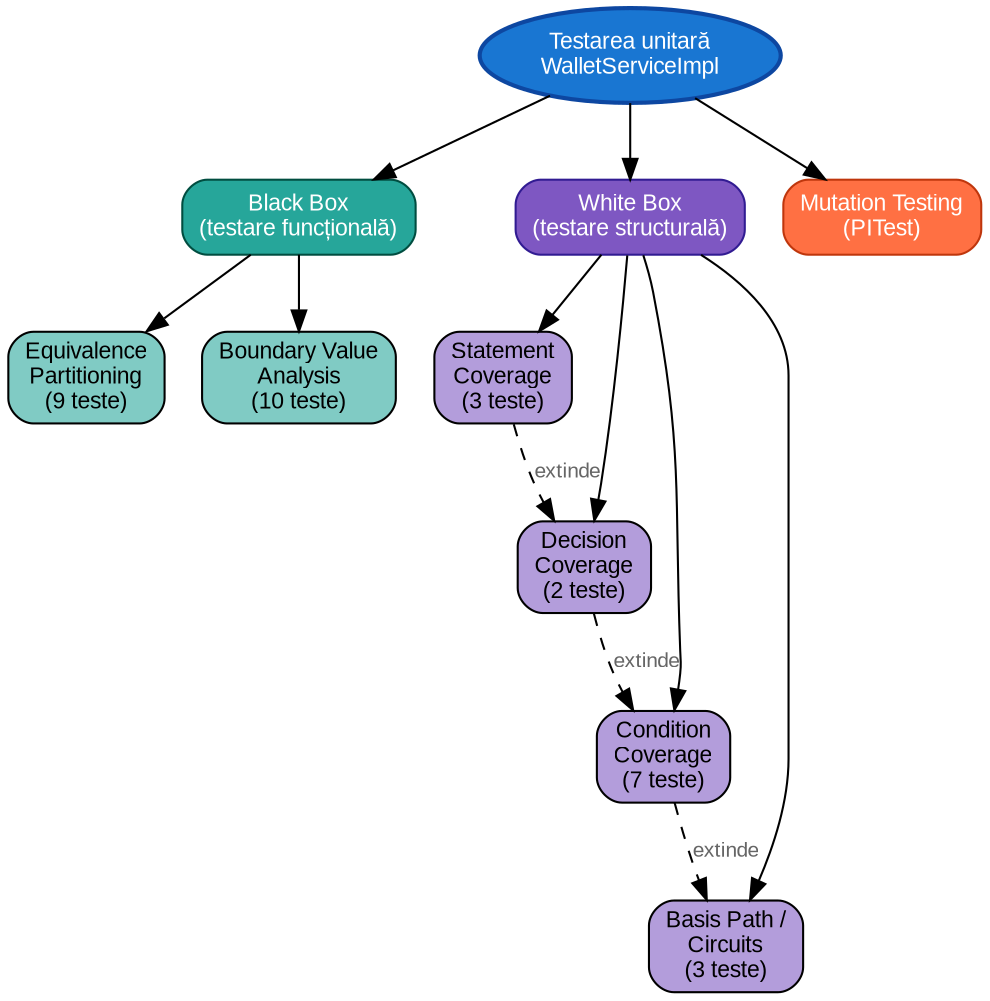
\includegraphics[width=0.85\linewidth]{07-strategies.png}
    \caption{Ierarhia strategiilor de testare aplicate în proiect, organizate pe ramurile Black Box / White Box / Mutation, cu numărul de teste scrise pentru fiecare strategie.}
    \label{fig:strategies}
\end{figure}

\subsection{Mutation Testing}

A treia familie - care nu e nici Black Box, nici White Box clasic - este \textit{Mutation Testing}. Aici nu se testează comportamentul codului, ci se testează \textit{calitatea testelor înseși} \cite{fmi_mutation_2024, pitest_docs}.

Metoda funcționează astfel: instrumentul (în cazul nostru \textsc{PITest}) creează în mod automat copii \textit{mutate} ale codului sursă - de exemplu, schimbă \texttt{>} cu \texttt{>=}, înlocuiește \texttt{||} cu \texttt{\&\&}, neagă o condiție - și rulează testele tale pe fiecare copie. Dacă măcar un test cade, mutația e considerată \textit{omorâtă}: înseamnă că suita a detectat alterarea. Dacă toate testele trec, mutația \textit{a supraviețuit}: a trecut prin testele tale fără să fie detectată, ceea ce înseamnă o lacună în suită.

\textit{Mutation score} = procentul de mutanți omorâți din totalul mutanților generați.

Scorul de mutation e o metrică mult mai severă decât \textit{statement} sau \textit{branch coverage}, pentru că poate evidenția situații în care testele \textit{ating} codul, dar nu îl \textit{verifică} - de exemplu, un test care doar invocă o metodă fără să facă niciun \texttt{assert} pe rezultat.

\section{Statement coverage}

\textit{Statement Coverage} este criteriul cel mai relaxat dintre cele structurale: cere doar ca fiecare linie de cod (mai exact, fiecare \textit{instrucțiune executabilă}) să fie executată cel puțin o dată de teste. Nu cere ca toate ramurile if/else să fie acoperite.

Exemplu - dat fragmentul:

\begin{lstlisting}[language=Java]
if (amount == null || amount.compareTo(BigDecimal.ZERO) <= 0) {
    throw new IllegalArgumentException("Suma trebuie sa fie > 0");
}
\end{lstlisting}

Pentru \textit{Statement Coverage} e suficient un singur test care intră pe ramura adevărată (de exemplu \texttt{amount = null}). Linia \texttt{throw} e executată, deci toate instrucțiunile sunt acoperite. Dar nu am testat ce se întâmplă în cazul \texttt{amount = 100} - am ratat ramura falsă.

\section{Decision coverage}

\textit{Decision Coverage} este criteriul \textit{branch}: pentru fiecare decizie din cod, atât rezultatul \textit{TRUE} cât și \textit{FALSE} trebuie să fi fost observate. La exemplul anterior, pentru a satisface Decision Coverage, avem nevoie de cel puțin două teste: unul cu \texttt{amount = null} (intră pe \textit{TRUE}) și unul cu \texttt{amount = 100} (intră pe \textit{FALSE}).

Acesta este criteriul măsurat efectiv de JaCoCo în coloana \textit{Branches}. Un branch coverage de 100\% nu garantează absența bug-urilor, dar e un prag minim profesional rezonabil. Comunitatea Google raportează un nivel de coverage pe proiectele lor între 60\% și 70\%, în funcție de domeniu \cite{google_coverage}.

\section{Condition coverage}

\textit{Condition Coverage} merge un nivel mai jos decât Decision: pentru orice condiție compusă (cu \texttt{\&\&} sau \texttt{||}), fiecare sub-condiție trebuie evaluată separat pe \textit{TRUE} și pe \textit{FALSE}.

Importanța acestei distincții apare la condițiile cu mai mulți operanzi. De exemplu:

\begin{lstlisting}[language=Java]
if (wallet == null || tx.getId() == null
        || !Objects.equals(tx.getWallet().getId(), wallet.getId())) {
    throw new IllegalStateException("Nu ai acces la aceasta tranzactie.");
}
\end{lstlisting}

\textit{Decision Coverage} se mulțumește cu două teste: unul în care expresia totală e adevărată (oricare din cele trei sub-condiții poate fi adevărată) și unul în care e falsă (toate sunt false). \textit{Condition Coverage} cere însă ca fiecare din cele trei sub-condiții să fie observată \textit{TRUE} și \textit{FALSE}, ceea ce duce la cel puțin 4 teste distincte.

\subsection{Short-circuit-ul Java}

Java evaluează operatorii \texttt{||} și \texttt{\&\&} cu \textit{short-circuit}: dacă primul operand poate decide rezultatul, al doilea nu mai e evaluat. La \texttt{||}, dacă primul e \textit{TRUE}, restul nu se mai evaluează. La \texttt{\&\&}, dacă primul e \textit{FALSE}, restul nu se mai evaluează.

În practică, asta înseamnă că pentru o condiție \texttt{a || b} cu doi operanzi, nu putem genera toate cele patru combinații posibile - \texttt{(T,T), (T,F), (F,T), (F,F)} - pentru că în primele două perechi, valoarea lui \texttt{b} nu se evaluează niciodată. Vom avea practic doar trei cazuri distincte:

\begin{enumerate}
    \item \texttt{a = TRUE} (b nu contează, e short-circuitat)
    \item \texttt{a = FALSE, b = TRUE}
    \item \texttt{a = FALSE, b = FALSE}
\end{enumerate}

Acest detaliu e important atunci când planificăm testele pentru condiții compuse - nu avem voie să cerem combinații imposibile.

\section{Basis Path Coverage (Circuits)}

\textit{Basis Path Coverage}, sau acoperirea pe \textit{circuite independente}, e cel mai sofisticat criteriu structural. Aici nu mai privim deciziile individual, ci la fluxul de control al metodei ca un întreg.

Pentru fiecare metodă, construim \textit{Control Flow Graph}-ul (CFG): un graf orientat în care nodurile sunt blocuri liniare de cod, iar muchiile sunt transferuri de control (ramuri \texttt{if}, return-uri, throw-uri).

Pentru un graf CFG, definim \textit{complexitatea ciclomatică} a lui McCabe \cite{mccabe1976} ca:

\begin{equation}
V(G) = E - N + 2
\end{equation}

unde $E$ este numărul de muchii și $N$ numărul de noduri. O formulă echivalentă, mai practică:

\begin{equation}
V(G) = \text{numărul de predicate} + 1
\end{equation}

\textit{Complexitatea ciclomatică} reprezintă numărul minim de \textit{căi independente} prin graf, adică numărul minim de teste necesare pentru a parcurge orice combinație de ramuri.

\textbf{Exemplu.} Pentru metoda \texttt{computeDaysRemainingSafe} din clasa noastră, CFG-ul are 8 noduri și 12 muchii (vezi figura \ref{fig:cfg-days}). Aplicând formula:

\begin{equation*}
V(G) = 12 - 8 + 2 = 6
\end{equation*}

Deci avem nevoie de cel puțin 6 teste pentru a parcurge toate căile independente. Aceste 6 căi corespund celor 6 scenarii distincte din metodă: \texttt{start = null}, \texttt{end = null}, interval invalid, călătorie încheiată, călătorie viitoare, călătorie în desfășurare.

\section{Mutation Testing - operatori și interpretare}

\textsc{PITest} suportă mai multe seturi de operatori de mutație. Pentru proiectul nostru am folosit setul \textit{STRONGER}, care e mai cuprinzător decât setul implicit \cite{pitest_mutators}. Cele mai relevante categorii de mutatori sunt:

\begin{description}
    \item[\textbf{ConditionalsBoundaryMutator}] - schimbă operatorii \texttt{<} cu \texttt{<=}, \texttt{>} cu \texttt{>=} și invers. E mutatorul cel mai eficient pentru a forța testele să distingă valorile exacte de pe granițe.

    \item[\textbf{NegateConditionalsMutator}] - inversează condițiile (de ex. \texttt{a == b} devine \texttt{a != b}). Verifică dacă testele detectează inversarea logică.

    \item[\textbf{MathMutator}] - schimbă operatorii aritmetici: \texttt{+} cu \texttt{-}, \texttt{*} cu \texttt{/} etc. Util pentru verificarea calculelor matematice.

    \item[\textbf{NullReturnValsMutator}] - face metodele să returneze \texttt{null}. Verifică dacă testele detectează valori nule pe care nu le-ar fi așteptat.

    \item[\textbf{VoidMethodCallMutator}] - șterge apelul la o metodă \texttt{void}. Util pentru a verifica dacă side-effect-urile sunt observate de teste (de exemplu, prin \texttt{verify()} pe mock-uri).

    \item[\textbf{RemoveConditionalMutator}] - elimină complet condiția (transformă \texttt{if (cond)} în \texttt{if (true)} sau \texttt{if (false)}). Are două variante: \textit{EQUAL} pentru egalități, \textit{ORDER} pentru comparații.
\end{description}

\subsection{Mutanți echivalenți}

Un caz important pe care literatura îl tratează cu seriozitate este al \textit{mutanților echivalenți} \cite{papadakis2019}. Un mutant e echivalent dacă, deși codul a fost modificat sintactic, comportamentul lui rămâne identic cu al codului original pentru orice intrare. Astfel de mutanți nu pot fi omorâți de niciun test, pentru că nu există un test care să producă vreo diferență observabilă.

Exemplu trivial: într-un \texttt{for} care iterează exact o dată, schimbarea limitei superioare cu o valoare mai mare (dar tot < \texttt{Integer.MAX\_VALUE}) nu schimbă nimic dacă bucla iese după prima iterație printr-un \texttt{break}. Un astfel de mutant supraviețuiește pentru că, semantic, codul a rămas același.

Distincția între mutanți \textit{neechivalenți} (care \textit{pot} fi omorâți și deci indică o lacună reală în suită) și \textit{echivalenți} (pe care îi documentăm ca atare) e o parte importantă a lucrului cu Mutation Testing. Cerința T3 cere explicit identificarea și omorârea a cel puțin doi mutanți neechivalenți.

\section{JaCoCo - cum măsoară coverage-ul}

JaCoCo \cite{jacoco_docs} e instrumentul standard pentru măsurarea coverage-ului în Java. Funcționează prin \textit{instrumentare la nivel de bytecode}: înainte de rularea testelor, modifică clasele compilate pentru a injecta sonde (\textit{probes}) care înregistrează ce instrucțiuni s-au executat.

Avantajul instrumentării bytecode-ului față de instrumentarea la nivelul codului sursă este precizia: JaCoCo măsoară exact ce s-a executat la nivelul JVM, nu o aproximare bazată pe linii de cod. În plus, raportul final indică nu doar instrucțiunile acoperite, ci și ramurile (\textit{branches}), liniile complexe, metodele atinse și clasele. Pentru proiectul nostru, urmărim în special:

\begin{itemize}
    \item \textbf{Instructions Coverage} - corespunde aproximativ noțiunii teoretice de \textit{Statement Coverage}, dar la nivel de bytecode.
    \item \textbf{Branches Coverage} - corespunde direct \textit{Decision Coverage}.
\end{itemize}

\section{De ce JUnit 5 + Mockito + JaCoCo + PITest}

Stiva de instrumente folosită este combinația standard în ecosistemul Java profesional \cite{junit_docs}. Toate cele patru instrumente sunt mature, bine documentate și se integrează unele cu altele:

\begin{itemize}
    \item \textbf{JUnit 5} (modulul Jupiter) e framework-ul principal de testare. Permite scrierea testelor cu adnotări (\texttt{@Test}, \texttt{@BeforeEach}), sistem de extensii (\texttt{@ExtendWith}) și asserțiuni declarative (\texttt{assertEquals}, \texttt{assertThrows}).
    \item \textbf{Mockito} se integrează cu JUnit 5 prin \texttt{MockitoExtension} și permite mock-uirea dependențelor cu \texttt{@Mock} și injectarea lor cu \texttt{@InjectMocks}.
    \item \textbf{JaCoCo} se integrează ca plugin Maven și instrumentează automat clasele înainte de rularea testelor.
    \item \textbf{PITest} se integrează tot ca plugin Maven și folosește testele JUnit existente pentru a evalua mutațiile.
\end{itemize}

În capitolele următoare, prezentăm aplicarea efectivă a acestor concepte pe clasa \texttt{WalletServiceImpl}.

\chapter{Configurația de lucru}
\label{ch:configurare}

În acest capitol descriem configurația concretă pe care a fost dezvoltat și testat proiectul: hardware, sistem de operare, alegerea de a nu folosi mașină virtuală, și versiunile exacte ale instrumentelor.

\section{Hardware}

Dezvoltarea s-a desfășurat în principal pe stația de lucru personală a șefei de echipă, cu următoarele specificații:

\begin{table}[!htb]
\centering
\caption{Configurația hardware folosită pentru dezvoltare și testare.}
\label{tab:hardware}
\begin{tabular}{ll}
\toprule
\textbf{Componentă} & \textbf{Specificație} \\
\midrule
Procesor & Intel Core i7-11800H, 8 nuclee, 16 fire, 2.30 GHz \\
Memorie RAM & 16 GB DDR4 \\
Stocare & SSD NVMe 512 GB \\
Placă video & NVIDIA GeForce RTX 3050 (4 GB) \\
\bottomrule
\end{tabular}
\end{table}

Cele trei membre ale echipei au folosit configurații similare, toate suficient de puternice pentru rularea suitei de teste și a instrumentelor de coverage. Suita completă (\texttt{mvn test}) rulează în aproximativ 2-3 secunde, iar PITest, care e cel mai costisitor, durează între 5 și 15 minute pentru cei 211 mutanți generați.

\section{Sistem de operare și mașini virtuale}

Sistemul de operare folosit a fost \textbf{Windows 11 Pro} (build 22H2), cu \textbf{PowerShell} ca shell pentru rularea comenzilor Maven. Comenzile sunt portabile și pe Linux/macOS dacă proiectul ar fi clonat acolo - Maven Wrapper (\texttt{mvnw}) e inclus în repository și are atât versiune \texttt{.cmd} pentru Windows, cât și script Unix.

\textbf{Nu a fost folosită nicio mașină virtuală.} Toate instrumentele (JDK, Maven, IntelliJ IDEA, Postgres pentru rularea aplicației) au fost instalate nativ pe Windows. Decizia a fost luată din considerente de performanță: rularea unei suite de teste cu Mockito e ușor afectată de overhead-ul unei VM, iar pentru PITest - care rulează \texttt{n} variante mutate ale codului, fiecare cu suita completă - timpul total ar fi crescut semnificativ.

Pentru baza de date am folosit \textbf{PostgreSQL 16} pentru aplicație și \textbf{H2 in-memory} pentru cazurile în care a fost nevoie să rulăm aplicația fără backend extern. Atenție însă: testele unitare nu folosesc nici Postgres, nici H2 - dependențele sunt complet mock-uite cu Mockito, deci suita rulează independent de orice bază de date.

\section{Stiva tehnologică}

Aplicația \textit{Călătorii} e construită pe Java 17 și Spring Boot 3.3.4. Tabelul \ref{tab:stack} sintetizează componentele majore.

\begin{table}[!htb]
\centering
\caption{Stiva tehnologică a aplicației și a suitei de teste.}
\label{tab:stack}
\begin{tabular}{lll}
\toprule
\textbf{Categorie} & \textbf{Tool / framework} & \textbf{Versiune} \\
\midrule
Limbaj & Java (OpenJDK) & 17 \\
Framework principal & Spring Boot & 3.3.4 \\
ORM & Hibernate (prin Spring Data JPA) & 6.5.x \\
Templating & Thymeleaf & 3.1.2 \\
Bază de date (prod) & PostgreSQL & 16 \\
Bază de date (dev) & H2 in-memory & 2.x \\
Build tool & Maven & 3.9.11 (prin wrapper) \\
Generare cod & Lombok & 1.18.42 \\
\midrule
Test framework & JUnit Jupiter & 5.10.3 \\
Mocking & Mockito (\texttt{mockito-junit-jupiter}) & 5.11.0 \\
Coverage & JaCoCo (Maven plugin) & 0.8.11 \\
Mutation Testing & PITest (\texttt{pitest-maven}) & 1.16.3 \\
\midrule
IDE & IntelliJ IDEA Ultimate & 2024.3.5 \\
Sistem de control versiuni & Git & 2.45.x \\
Hosting repo & GitHub & N/A \\
\bottomrule
\end{tabular}
\end{table}

\subsection{Justificarea alegerii instrumentelor de testare}

Stiva \textit{JUnit 5 + Mockito + JaCoCo + PITest} este, de facto, standardul pentru testare unitară pe ecosistemul Java în 2026. Câteva motive concrete pentru fiecare alegere:

\paragraph{JUnit 5 (Jupiter)} este versiunea modernă, modulară, a JUnit-ului. Față de JUnit 4 oferă: metode de test \texttt{package-private} (nu mai trebuie \texttt{public}), un sistem de extensii curat prin \texttt{@ExtendWith}, asserțiuni îmbunătățite (\texttt{assertThrows}, \texttt{assertAll}), suport nativ pentru parametrizate. Vine implicit prin \texttt{spring-boot-starter-test}, deci nu trebuie adăugat manual.

\paragraph{Mockito} este alegerea standard pentru mock-uri în Java, cu o sintaxă fluentă (\texttt{when(...).thenReturn(...)}) și integrare elegantă cu JUnit 5. Alternativele - EasyMock, PowerMock - sunt fie mai vechi, fie au probleme cu noile versiuni de Java.

\paragraph{JaCoCo} este, de asemenea, instrumentul standard în ecosistemul Java, integrat cu Maven, Gradle și majoritatea IDE-urilor. Generează rapoarte HTML interactive în care fiecare linie e colorată în verde (acoperită), galben (parțial acoperită) sau roșu (neatinsă).

\paragraph{PITest} este instrumentul lider pentru Mutation Testing pe Java, cu performanță bună și un set bogat de mutatori. Alternativele (\textit{MuJava}, \textit{Major}) sunt mai academice, mai puțin întreținute și mai dificil de integrat cu Maven.

\section{Arhitectura proiectului}

Aplicația respectă structura clasică \textit{layered} a unui proiect Spring Boot, vizibilă în figura \ref{fig:architecture}:

\begin{figure}[!htb]
    \centering
    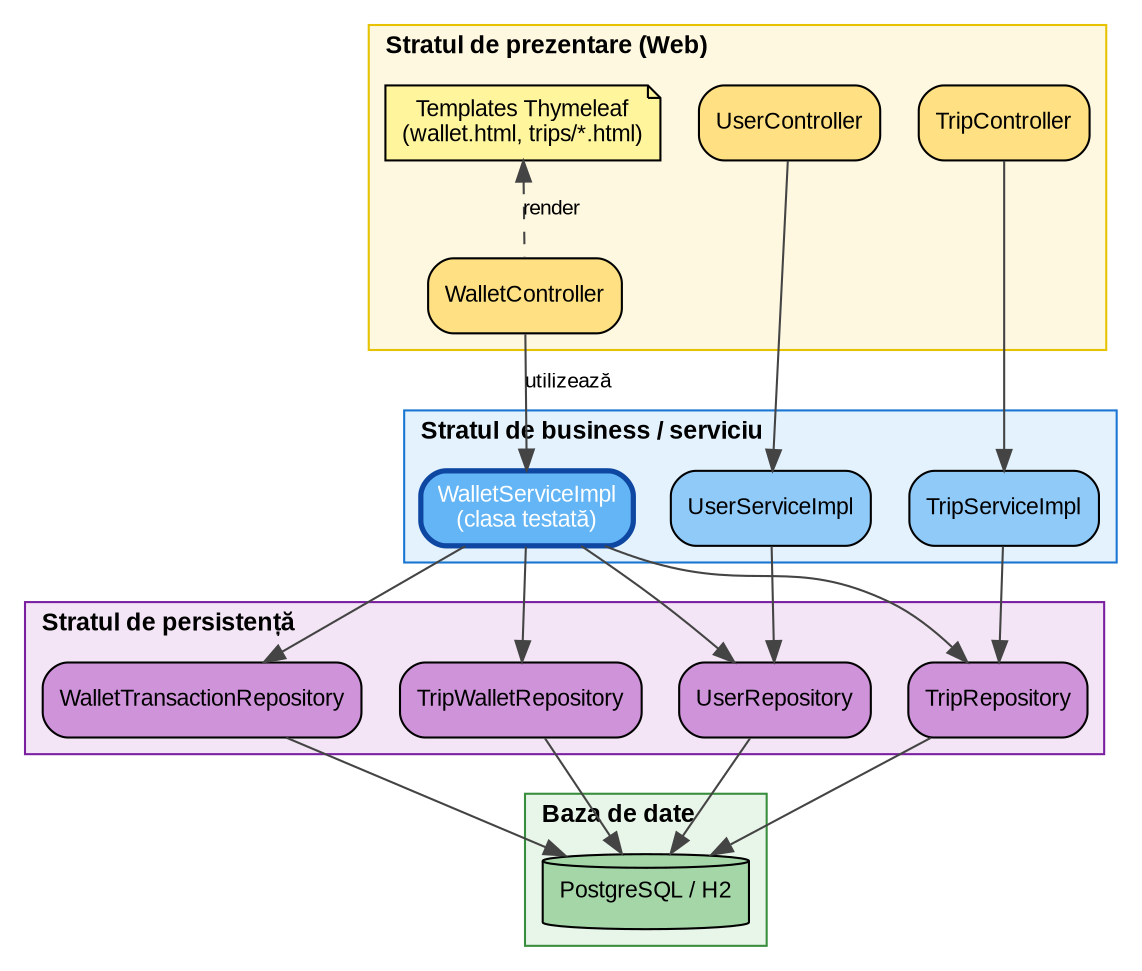
\includegraphics[width=0.9\linewidth]{01-architecture.png}
    \caption{Arhitectura aplicației \textit{Călătorii} pe trei straturi (prezentare, business, persistență), cu evidențierea clasei testate \texttt{WalletServiceImpl}.}
    \label{fig:architecture}
\end{figure}

\begin{itemize}
    \item \textbf{Stratul de prezentare} - controllere Spring MVC + template-uri Thymeleaf. Pentru wallet, există un singur \texttt{WalletController} care expune endpoint-urile HTTP.
    \item \textbf{Stratul de business} - serviciile cu logica aplicativă. \texttt{WalletServiceImpl} e implementarea concretă a interfeței \texttt{WalletService} și e clasa pe care o testăm în acest proiect.
    \item \textbf{Stratul de persistență} - patru repository-uri JPA pe care \texttt{WalletServiceImpl} le folosește prin injecție de dependențe: \texttt{TripRepository}, \texttt{TripWalletRepository}, \texttt{UserRepository}, \texttt{WalletTransactionRepository}.
    \item \textbf{Baza de date} - PostgreSQL pentru rularea efectivă a aplicației.
\end{itemize}

În testele unitare, întreg stratul de persistență e mock-uit, ceea ce face ca testele să fie rapide și deterministe.

\section{Configurarea Maven (pom.xml)}

Plugin-urile principale relevante pentru testare sunt configurate în \texttt{pom.xml} astfel.

Pentru \textbf{JaCoCo}:

\begin{lstlisting}[language=XML, caption={Configurarea pluginului JaCoCo în pom.xml.}]
<plugin>
    <groupId>org.jacoco</groupId>
    <artifactId>jacoco-maven-plugin</artifactId>
    <version>0.8.11</version>
    <executions>
        <execution>
            <id>prepare-agent</id>
            <goals>
                <goal>prepare-agent</goal>
            </goals>
        </execution>
        <execution>
            <id>report</id>
            <phase>test</phase>
            <goals>
                <goal>report</goal>
            </goals>
            <configuration>
                <includes>
                    <include>echipa13/calatorii/service/impl/WalletServiceImpl.class</include>
                </includes>
            </configuration>
        </execution>
    </executions>
</plugin>
\end{lstlisting}

Filtrul \texttt{includes} limitează raportul JaCoCo la o singură clasă - \texttt{WalletServiceImpl}. Decizia e deliberată: cerința proiectului e să testăm o singură clasă reprezentativă, iar dacă raportul ar include toată aplicația, procentele ar fi diluate de codul netestat din celelalte module.

Pentru \textbf{PITest}:

\begin{lstlisting}[language=XML, caption={Configurarea pluginului PITest în pom.xml.}]
<plugin>
    <groupId>org.pitest</groupId>
    <artifactId>pitest-maven</artifactId>
    <version>1.16.3</version>
    <dependencies>
        <dependency>
            <groupId>org.pitest</groupId>
            <artifactId>pitest-junit5-plugin</artifactId>
            <version>1.2.2</version>
        </dependency>
    </dependencies>
    <configuration>
        <targetClasses>
            <param>echipa13.calatorii.service.impl.WalletServiceImpl</param>
        </targetClasses>
        <targetTests>
            <param>echipa13.calatorii.service.impl.WalletServiceImpl*Test</param>
        </targetTests>
        <outputFormats>
            <outputFormat>HTML</outputFormat>
            <outputFormat>XML</outputFormat>
        </outputFormats>
        <mutators>
            <mutator>STRONGER</mutator>
        </mutators>
    </configuration>
</plugin>
\end{lstlisting}

Setul de mutatori \texttt{STRONGER} extinde setul implicit (\texttt{DEFAULTS}) cu mutatori suplimentari: \textit{InlineConstantMutator}, \textit{NonVoidMethodCallMutator}, \textit{ExperimentalSwitchMutator} etc. Decizia de a folosi setul mai complet a fost luată pentru că vrem un raport care să stresseze cât mai mult suita.

Plugin-ul \texttt{pitest-junit5-plugin} e necesar deoarece varianta de bază a PITest înțelege doar JUnit 4. Trebuie declarat ca dependență internă a plugin-ului.

\section{Versiunea de Java și note de compatibilitate}

Proiectul rulează pe \textbf{Java 17} (LTS), care este versiunea minimă cerută de Spring Boot 3.x. Pe stațiile de dezvoltare, JDK-ul efectiv folosit a fost \textbf{OpenJDK 24}, care e backwards-compatible cu Java 17.

O incompatibilitate pe care am întâlnit-o în timpul setup-ului: versiunea standard de Lombok (1.18.32) nu funcționa cu OpenJDK 24, returnând erori de \textit{annotation processing}. Soluția a fost să forțăm explicit Lombok 1.18.42 (ultima versiune stabilă la momentul predării proiectului) prin \texttt{annotationProcessorPaths} în \texttt{maven-compiler-plugin}.

În capitolul următor descriem aplicația \textit{Călătorii} și clasa \texttt{WalletServiceImpl}, înainte de a intra în detaliile testării propriu-zise.

\chapter{Aplicația și clasa testată}
\label{ch:aplicatia}

\section{Aplicația \textit{Călătorii}}

\textit{Călătorii} este o aplicație web de planificare și jurnalizare a vacanțelor, dezvoltată de echipa noastră ca proiect personal pe parcursul anului. Aplicația permite utilizatorilor să:

\begin{itemize}
    \item creeze itinerarii multi-day (\textit{trips}) cu titlu, dată de început, dată de sfârșit, descriere și categorie;
    \item adauge un \textit{jurnal} pe fiecare zi - notițe, poze, locații vizitate;
    \item cumpere \textit{tururi} create de ghizi din comunitate (folosind un sistem de puncte fictiv);
    \item urmărească pe o hartă interactivă țările vizitate;
    \item urmărească alte profiluri de utilizator și să interacționeze prin urmăriri (\textit{follow}-uri);
    \item discute cu un \textit{chatbot} despre destinații și recomandări;
    \item \textbf{gestioneze bugetul fiecărei călătorii} (modulul \textit{Wallet} - cel pe care îl testăm).
\end{itemize}

Aplicația are aproximativ 25 de entități JPA, 15 controllere Spring MVC și peste 30 de template-uri Thymeleaf. Pentru proiectul T3, am ales un singur modul reprezentativ - \textit{Wallet} - pe care să aplicăm testarea unitară completă.

\section{Modulul Wallet - context și roluri}

Fiecare călătorie (\texttt{Trip}) are asociat un singur portofel (\texttt{TripWallet}), legat printr-o relație 1-la-1 prin foreign key. Portofelul are un buget total și o monedă (RON sau EUR), iar utilizatorul poate adăuga \textit{tranzacții} (\texttt{WalletTransaction}) pentru fiecare cheltuială făcută în călătorie.

Rolul aplicativ al modulului este să răspundă la întrebări de tipul:

\begin{itemize}
    \item Câți bani am alocat pentru această vacanță?
    \item Cât am cheltuit până acum, pe categorii (mâncare, transport, cazare, suveniruri etc.)?
    \item Sunt în limita bugetului sau aproape de a-l depăși?
    \item Cu ritmul curent de cheltuieli, în câte zile voi epuiza bugetul?
    \item Cât îmi mai pot permite să cheltui pe zi pentru a rămâne în buget?
\end{itemize}

Răspunsurile la aceste întrebări sunt calculate de \texttt{WalletServiceImpl} pe baza datelor din baza de date. Răspunsurile sunt apoi afișate în interfață într-o pagină dedicată, cu KPI-uri colorate, grafice de cheltuieli pe categorii și un mesaj de recomandare în limba română.

\section{Diagrama claselor}

Figura \ref{fig:classes} prezintă diagrama claselor implicate în modulul Wallet, cu \texttt{WalletServiceImpl} în centru și entitățile JPA cu care interacționează.

\begin{figure}[!htb]
    \centering
    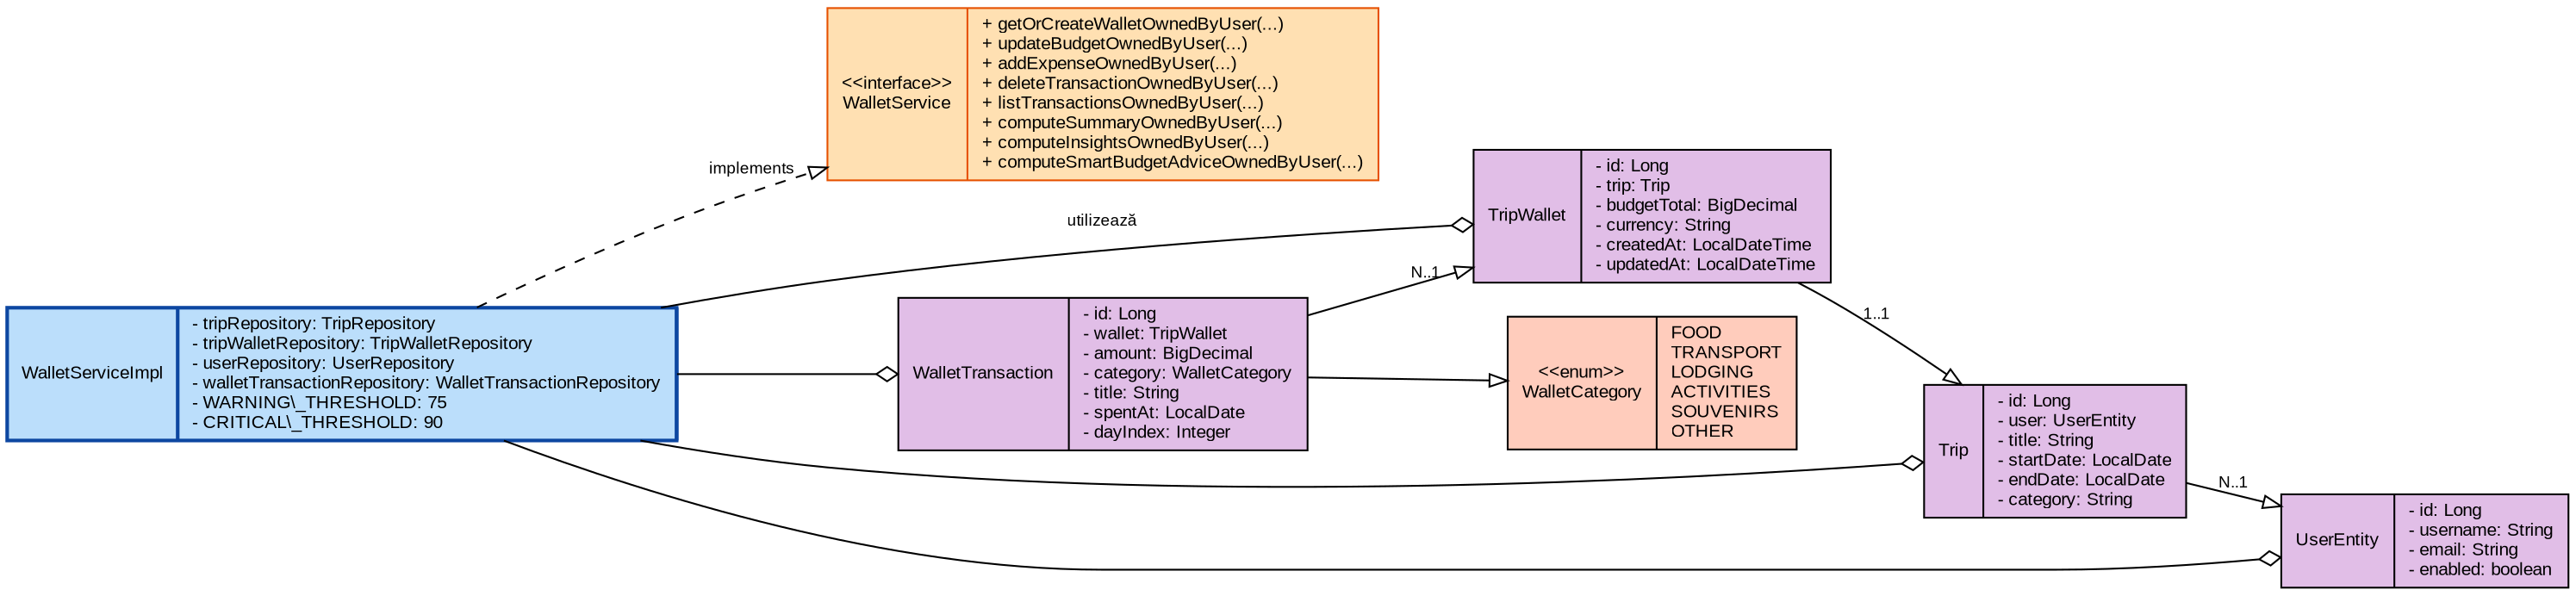
\includegraphics[width=\linewidth]{02-classes.png}
    \caption{Diagrama claselor pentru modulul Wallet, cu accent pe \texttt{WalletServiceImpl} - clasa testată.}
    \label{fig:classes}
\end{figure}

Câteva observații din diagramă:

\begin{itemize}
    \item \texttt{WalletServiceImpl} implementează interfața \texttt{WalletService} (programare orientată pe contract).
    \item Are patru dependențe injectate prin constructor (toate sunt repository-uri JPA): \texttt{TripRepository}, \texttt{TripWalletRepository}, \texttt{UserRepository}, \texttt{WalletTransactionRepository}.
    \item \texttt{TripWallet} are relație 1-la-1 cu \texttt{Trip}, iar \texttt{Trip} are relație N-la-1 cu \texttt{UserEntity} (un user poate avea mai multe călătorii).
    \item \texttt{WalletTransaction} are relație N-la-1 cu \texttt{TripWallet} (un portofel poate avea multe tranzacții) și folosește un enum \texttt{WalletCategory} cu șase valori (FOOD, TRANSPORT, LODGING, ACTIVITIES, SOUVENIRS, OTHER).
\end{itemize}

\section{Clasa \texttt{WalletServiceImpl} - prezentare}

\texttt{WalletServiceImpl} este o clasă de aproximativ 435 de linii, cu 21 de metode publice și 7 metode private. Complexitatea ciclomatică McCabe a metodelor variază între 1 (getters/setters automate) și 18 (metoda \texttt{buildRecommendation}, care construiește textul recomandării pe baza mai multor condiții).

\subsection{Metodele publice principale}

Tabelul \ref{tab:methods} listează metodele publice și, pentru fiecare, descrierea succintă și complexitatea ciclomatică estimată.

\begin{table}[!htb]
\centering
\caption{Metodele publice din \texttt{WalletServiceImpl}, ordonate după complexitate.}
\label{tab:methods}
\begin{tabularx}{\linewidth}{lXc}
\toprule
\textbf{Metodă} & \textbf{Descriere} & \textbf{V(G)} \\
\midrule
\texttt{computeSmartBudgetAdvice...} & Generează sfat inteligent: ritm, allowance, forecast & 18 \\
\texttt{computeSummaryOwnedByUser} & KPI buget: total / cheltuit / status & 5 \\
\texttt{computeInsightsOwnedByUser} & Insights pe categorii și zile active & 6 \\
\texttt{addExpenseOwnedByUser} & Adaugă cheltuială cu validări & 4 \\
\texttt{deleteTransaction...} & Șterge tranzacție cu verificare ownership & 4 \\
\texttt{updateBudgetOwnedByUser} & Actualizează buget cu validări & 5 \\
\texttt{getOrCreateWallet...} & Returnează portofelul sau îl creează & 2 \\
\texttt{listTransactions...} & Listează tranzacțiile sortate & 1 \\
\bottomrule
\end{tabularx}
\end{table}

Metodele \texttt{...OwnedByUser} primesc întotdeauna ca parametru un \texttt{login} (email sau username), iar prima operațiune internă pe care o fac este să verifice că utilizatorul curent are acces la călătoria respectivă. Aceasta e logica de \textit{ownership check}, esențială pentru securitatea aplicației.

\subsection{Logica de ownership check}

Înainte de orice operație, \texttt{WalletServiceImpl} verifică două lucruri:

\begin{enumerate}
    \item Utilizatorul cu login-ul dat există în baza de date.
    \item Călătoria cu \texttt{tripId} dat aparține efectiv acestui utilizator.
\end{enumerate}

Codul concret e următorul:

\begin{lstlisting}[language=Java, caption={Logica de ownership check.}]
private Trip getTripOwnedByUser(Long tripId, String usernameOrEmail) {
    UserEntity user = findUserByUsernameOrEmail(usernameOrEmail)
        .orElseThrow(() -> new IllegalArgumentException(
            "Utilizator inexistent."));

    Trip trip = tripRepository.findById(tripId)
        .orElseThrow(() -> new IllegalArgumentException(
            "Itinerariu inexistent."));

    if (trip.getUser() == null
            || !Objects.equals(trip.getUser().getId(), user.getId())) {
        throw new IllegalStateException(
            "Nu ai acces la acest itinerariu.");
    }
    return trip;
}
\end{lstlisting}

Metoda are trei puncte de eșec posibile (utilizator inexistent, călătorie inexistentă, ownership greșit) care trebuie acoperite de teste pentru fiecare strategie aplicată.

\subsection{Pragurile dinamice și enum-ul de stare}

Una dintre cele mai testabile părți ale clasei este logica de \textit{stare a bugetului}, care folosește un enum cu 4 valori și două praguri configurabile:

\begin{lstlisting}[language=Java, caption={Pragurile și enum-ul Status.}]
private static final int WARNING_THRESHOLD_PERCENT  = 75;
private static final int CRITICAL_THRESHOLD_PERCENT = 90;

public enum Status {
    NESETAT, OK, ATENTIE, DEPASIT
}
\end{lstlisting}

Logica de stare:

\begin{lstlisting}[language=Java]
if (percent >= 100)                     status = Status.DEPASIT;
else if (percent >= WARNING_THRESHOLD)  status = Status.ATENTIE;
else                                    status = Status.OK;
\end{lstlisting}

Această cascadă de praguri e un teren foarte fertil pentru \textbf{Boundary Value Analysis}: trebuie să verificăm cu testele exact valorile 74, 75, 99, 100 pentru a ne asigura că pragurile sunt setate corect și că relația \texttt{>=} e folosită corect (nu \texttt{>}).

\subsection{Buget inteligent (\textit{smart advice}) - extensie}

În plus față de calculul KPI clasic, am adăugat o metodă numită \texttt{computeSmartBudgetAdvice...} care folosește mai multe sub-metode pentru a calcula:

\begin{itemize}
    \item \textbf{burn rate per zi} - cheltuiala medie zilnică, calculată pe baza zilelor efective de consum;
    \item \textbf{daily allowance} - cât îți poți permite să cheltui pe zi pentru a rămâne în buget până la finalul călătoriei;
    \item \textbf{days to exceed} - estimarea numărului de zile până la depășirea bugetului, dacă ritmul actual continuă;
    \item \textbf{recommendation} - un text în română care sintetizează informațiile pentru utilizator.
\end{itemize}

Această metodă e cea cu cea mai mare complexitate ciclomatică (V(G) = 18), pentru că apelează intern alte trei metode private cu propriile decizii (\texttt{buildRiskUi}, \texttt{computeDaysRemainingSafe}, \texttt{buildRecommendation}). Tocmai din cauza complexității, o folosim ca subiect principal pentru \textit{Decision Coverage} și \textit{Condition Coverage}.

\section{De ce am ales \texttt{WalletServiceImpl} pentru testare}

În aplicația \textit{Călătorii} avem multiple clase de serviciu: \texttt{TripServiceImpl}, \texttt{UserServiceImpl}, \texttt{TourServiceImpl}, \texttt{LeaderboardServiceImpl} etc. Înainte de a alege \texttt{WalletServiceImpl}, am evaluat fiecare candidat după mai multe criterii:

\begin{table}[!htb]
\centering
\caption{Compararea claselor candidat pentru testare unitară.}
\label{tab:candidates}
\begin{tabularx}{\linewidth}{Xccccc}
\toprule
\textbf{Clasă} & \textbf{V(G) max} & \textbf{Cond. compuse} & \textbf{Calcule} & \textbf{Mockabil} & \textbf{Ales} \\
\midrule
\texttt{TripServiceImpl} & 4 & \(\times\) & \(\times\) & \checkmark & nu \\
\texttt{UserServiceImpl} & 6 & \(\times\) & \(\times\) & dificil & nu \\
\texttt{TourServiceImpl} & 5 & \checkmark & \(\times\) & \checkmark & nu \\
\texttt{LeaderboardServiceImpl} & 8 & \checkmark & \checkmark & \checkmark & nu \\
\texttt{WalletServiceImpl} & \textbf{18} & \textbf{\checkmark} & \textbf{\checkmark} & \textbf{\checkmark} & \textbf{da} \\
\bottomrule
\end{tabularx}
\end{table}

Motivele concrete pentru care am ales \texttt{WalletServiceImpl}:

\begin{enumerate}
    \item \textbf{Complexitate suficientă pentru toate cele șase strategii.} Are condiții compuse cu 2-3 operanzi (pentru Condition Coverage), cascade de \texttt{if}-uri pe praguri (pentru Decision Coverage), metode cu V(G) între 5 și 18 (pentru Circuits Coverage), și calcule cu \texttt{BigDecimal} (pentru Math Mutators în PITest).

    \item \textbf{Logică de business reală, nu CRUD trivial.} Clasa nu face doar \texttt{save} și \texttt{findById} - face validări, calcule pe rate, comparații pe praguri, generare de mesaje. Asta înseamnă că testele au valoare reală: prind bug-uri concrete.

    \item \textbf{Patru dependențe perfect mockable.} \texttt{WalletServiceImpl} primește toate dependențele prin constructor, ceea ce face Mockito-ul direct: \texttt{@Mock} + \texttt{@InjectMocks} și gata. Nu trebuie context Spring, nu trebuie bază de date.

    \item \textbf{Domeniul aplicativ e \enquote{financiar}.} Asta înseamnă că un bug în această clasă afectează direct percepția utilizatorului despre banii lui - ceea ce e mult mai grav decât un bug în layout-ul HTML. Logic, e exact tipul de cod care trebuie testat cu cea mai mare grijă.

    \item \textbf{Enum cu 4 stări.} \texttt{Status.\{NESETAT, OK, ATENTIE, DEPASIT\}} oferă un set finit, clar definit de comportamente posibile, ceea ce face testele deterministe și ușor de verificat.
\end{enumerate}

În capitolul următor prezentăm efectiv aplicarea celor șase strategii pe această clasă, cu exemple de cod, tabele și diagrame pentru fiecare.

\chapter{Strategiile de testare aplicate}
\label{ch:strategii}

În acest capitol prezentăm aplicarea efectivă a celor șase strategii de testare pe \texttt{WalletServiceImpl}, cu exemple de cod, tabele de partiții/frontiere/circuite și interpretări.

\section{Organizarea suitei}

Am ales să organizăm suita pe \textbf{șapte fișiere de test}, câte unul pentru fiecare strategie (plus unul pentru Mutation Testing):

\begin{table}[!htb]
\centering
\caption{Organizarea suitei de teste, pe strategii.}
\label{tab:test-files}
\begin{tabular}{lcl}
\toprule
\textbf{Fișier} & \textbf{Nr. teste} & \textbf{Strategie} \\
\midrule
\texttt{...EquivalenceTest.java} & 9 & Equivalence Partitioning \\
\texttt{...BoundaryTest.java} & 10 & Boundary Value Analysis \\
\texttt{...StatementTest.java} & 3 & Statement Coverage \\
\texttt{...DecisionTest.java} & 2 & Decision Coverage \\
\texttt{...ConditionTest.java} & 7 & Condition Coverage \\
\texttt{...CircuitsTest.java} & 3 & Basis Path / Circuits \\
\texttt{...MutationTest.java} & 5+ & Mutation Testing \\
\midrule
\textbf{Total} & \textbf{$\sim$40} & \\
\bottomrule
\end{tabular}
\end{table}

Distribuția vizuală e prezentată în figura \ref{fig:test-distribution}.

\begin{figure}[!htb]
    \centering
    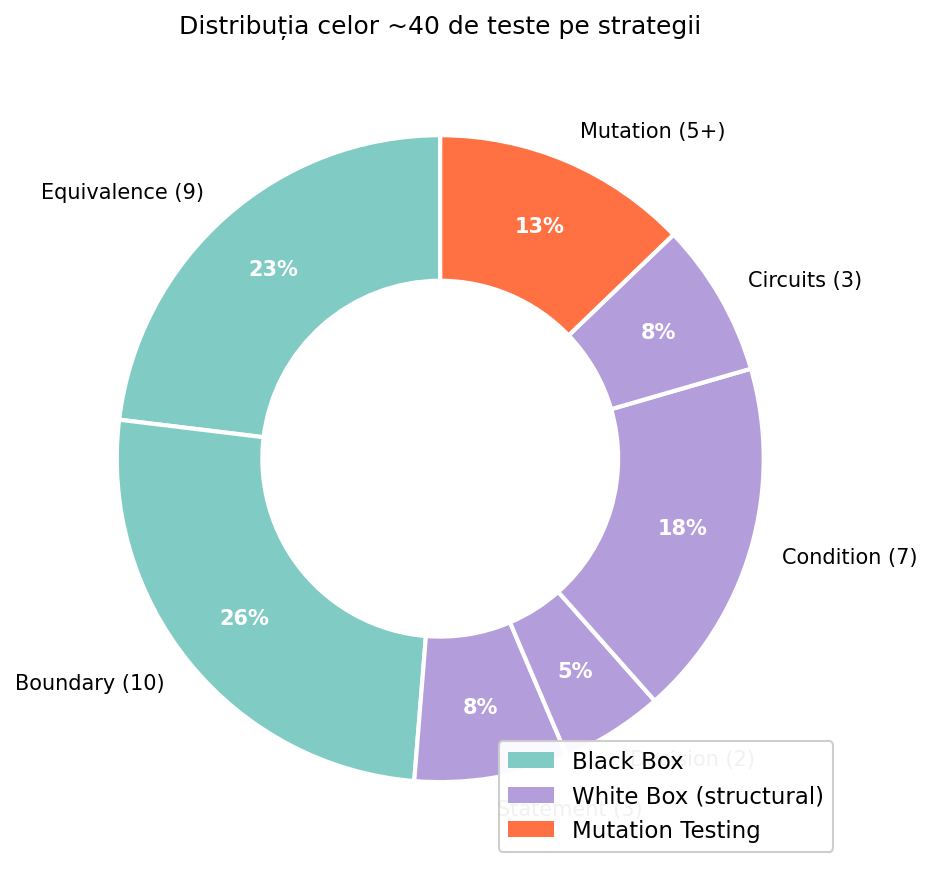
\includegraphics[width=0.7\linewidth]{12-test-distribution.png}
    \caption{Distribuția testelor pe cele șase strategii + Mutation. Culorile evidențiază clasificarea Black Box / White Box / Mutation.}
    \label{fig:test-distribution}
\end{figure}

\subsection{Decizia de a aplica strategiile pe metode diferite}

O decizie importantă în planificarea suitei a fost dacă să aplicăm \textit{toate} cele șase strategii pe \textit{aceeași} metodă, sau dacă să distribuim strategiile pe metodele cele mai potrivite. Am ales a doua variantă, din mai multe motive:

\begin{itemize}
    \item Nu toate metodele au sens pentru toate strategiile. \texttt{listTransactionsOwnedByUser}, de exemplu, are V(G) = 1 și o singură instrucțiune relevantă. Statement Coverage și Decision Coverage sunt triviale pe ea, iar Condition Coverage nu se aplică (nu există condiții compuse).
    \item Reflectă mai fidel practica profesională: un test bun se aplică acolo unde se aplică natural. Forțarea unei strategii pe un cod care nu o cere produce teste artificiale, care nu adaugă valoare.
    \item Distribuția a permis să acoperim 21 din 21 de metode publice ale clasei la coverage de 100\% (vezi capitolul \ref{ch:jacoco}), față de a ne fi concentrat pe 1-2 metode.
\end{itemize}

Tabelul \ref{tab:strategy-method} arată maparea strategie - metodă principal țintită.

\begin{table}[!htb]
\centering
\caption{Strategia aplicată și metoda principală țintită.}
\label{tab:strategy-method}
\begin{tabularx}{\linewidth}{lX}
\toprule
\textbf{Strategie} & \textbf{Metoda principală} \\
\midrule
Equivalence Partitioning & \texttt{addExpenseOwnedByUser} \\
Boundary Value Analysis & \texttt{addExpense...} + \texttt{computeSummary...} \\
Statement Coverage & \texttt{updateBudget...} + \texttt{deleteTransaction...} \\
Decision Coverage & \texttt{computeSmartBudgetAdvice...} \\
Condition Coverage & multiple metode cu condiții compuse \\
Circuits & \texttt{findUserBy...} + \texttt{computeDaysRemainingSafe} + \texttt{computeInsights...} \\
Mutation Testing & raport general + teste țintite pe mutanți \\
\bottomrule
\end{tabularx}
\end{table}

\section{Echipamentul comun de test (test fixture)}

Toate cele șapte fișiere folosesc o structură similară, cu mock-uri pe cele patru repository-uri și un fixture comun de utilizator + călătorie + portofel:

\begin{lstlisting}[language=Java, caption={Schelet comun pentru fișierele de test.}]
@ExtendWith(MockitoExtension.class)
@MockitoSettings(strictness = Strictness.LENIENT)
public class WalletServiceImplXxxTest {

    @Mock private TripRepository tripRepo;
    @Mock private TripWalletRepository walletRepo;
    @Mock private UserRepository userRepo;
    @Mock private WalletTransactionRepository txRepo;

    @InjectMocks private WalletServiceImpl service;

    private TripWallet wallet;
    private Trip trip;
    private final Long tripId = 10L;
    private final String login = "user@test.com";

    @BeforeEach
    public void setUp() {
        UserEntity user = new UserEntity();
        user.setId(1L);

        trip = new Trip();
        trip.setId(tripId);
        trip.setUser(user);

        wallet = new TripWallet();
        wallet.setTrip(trip);

        when(userRepo.findByEmail(login)).thenReturn(user);
        when(tripRepo.findById(tripId)).thenReturn(Optional.of(trip));
        when(walletRepo.findByTrip_Id(tripId)).thenReturn(Optional.of(wallet));
    }

    // teste specifice strategiei...
}
\end{lstlisting}

Adnotarea \texttt{@MockitoSettings(strictness = Strictness.LENIENT)} permite ca stub-urile declarate în \texttt{@BeforeEach} să nu fie folosite în fiecare test individual, fără ca Mockito să arunce eroarea \texttt{UnnecessaryStubbingException}. Asta e util pentru fixture-urile comune, care sunt folosite selectiv.

% --------------------------------------------------------------------
\section{Equivalence Partitioning}
\label{sec:ep}

\textit{Equivalence Partitioning} (EP) împarte spațiul de input al unei metode în clase echivalente, în care comportamentul așteptat e identic. Apoi alegem un singur reprezentant pe clasă.

\subsection{Metoda țintă: \texttt{addExpenseOwnedByUser}}

Metoda primește 6 parametri: \texttt{amount}, \texttt{category}, \texttt{title}, \texttt{note}, \texttt{spentAt}, \texttt{dayIndex}. Pentru fiecare am identificat clasele relevante.

\begin{table}[!htb]
\centering
\caption{Clase de echivalență pentru \texttt{addExpenseOwnedByUser}.}
\label{tab:ep-classes}
\begin{tabularx}{\linewidth}{clX}
\toprule
\textbf{Partiție} & \textbf{Condiție} & \textbf{Comportament așteptat} \\
\midrule
P1 & toate input-urile valide & \texttt{save()} pe \texttt{txRepo}, tranzacție creată corect \\
P2 & \texttt{category = null} & fallback la \texttt{WalletCategory.OTHER} \\
P3 & \texttt{spentAt = null} & fallback la \texttt{LocalDate.now()} \\
P4 & \texttt{amount} \texttt{null}/negativă & \texttt{IllegalArgumentException} \\
P5 & \texttt{title} blank/null & \texttt{IllegalArgumentException} \\
P6 & \texttt{dayIndex <= 0} & \texttt{IllegalArgumentException} \\
P7 & apel \texttt{listTransactions...} & lista sortată din repo \\
P8 & \texttt{tripId} inexistent & \texttt{IllegalArgumentException} \\
\bottomrule
\end{tabularx}
\end{table}

\subsection{Exemplu de test EP}

\begin{lstlisting}[language=Java, caption={Test pentru P2 - categorie nulă.}]
@Test
public void testAdaugaCheltuiala_CategorieLipsa() {
    // P2: categorie null -> fallback OTHER
    service.addExpenseOwnedByUser(tripId, login,
            new BigDecimal("25.00"), null, "Taxi", null,
            LocalDate.of(2026, 4, 18), 2);

    ArgumentCaptor<WalletTransaction> cap =
        ArgumentCaptor.forClass(WalletTransaction.class);
    verify(txRepo).save(cap.capture());
    assertEquals(WalletCategory.OTHER, cap.getValue().getCategory());
}
\end{lstlisting}

Folosim \texttt{ArgumentCaptor} pentru a captura argumentul cu care a fost apelată metoda \texttt{save()} pe mock, ca să verificăm că enum-ul a fost setat corect.

\subsection{Numărul de teste pentru EP}

În total, fișierul \texttt{...EquivalenceTest.java} conține \textbf{9 teste}, câte unul pentru fiecare partiție P1-P8, plus un test suplimentar care verifică că și \texttt{title = null} (nu doar \texttt{title} blank cu spații) e respins corect - o sub-partiție a P5.

% --------------------------------------------------------------------
\section{Boundary Value Analysis}
\label{sec:bva}

\textit{Boundary Value Analysis} (BVA) testează valori chiar pe granițe, nu doar reprezentanți tipici. Bug-urile cele mai frecvente apar exact la \texttt{<} vs. \texttt{<=}.

\subsection{Frontiere pentru \texttt{addExpenseOwnedByUser}}

\begin{table}[!htb]
\centering
\caption{Valorile de frontieră testate pentru \texttt{addExpenseOwnedByUser}.}
\label{tab:bva-input}
\begin{tabularx}{\linewidth}{lcXX}
\toprule
\textbf{Parametru} & \textbf{Val.} & \textbf{Validitate} & \textbf{Justificare} \\
\midrule
\texttt{amount} & 0 & invalid & exact pe pragul \texttt{<= 0} \\
\texttt{amount} & 0.01 & valid & cea mai mică valoare validă \\
\texttt{amount} & -10 & invalid & sub frontieră \\
\texttt{title} & "" & invalid & string gol \\
\texttt{title} & "a" & valid & cel mai scurt valid \\
\texttt{dayIndex} & 0 & invalid & exact pe \texttt{<= 0} \\
\texttt{dayIndex} & 1 & valid & primul valid \\
\bottomrule
\end{tabularx}
\end{table}

\subsection{Frontiere pentru cascada de praguri}

Cea mai relevantă aplicare a BVA e pe metoda \texttt{computeSummaryOwnedByUser}, care folosește praguri la 75\% și 100\% pentru a stabili \texttt{Status}. Figura \ref{fig:thresholds} arată grafic cascada și valorile testate.

\begin{figure}[!htb]
    \centering
    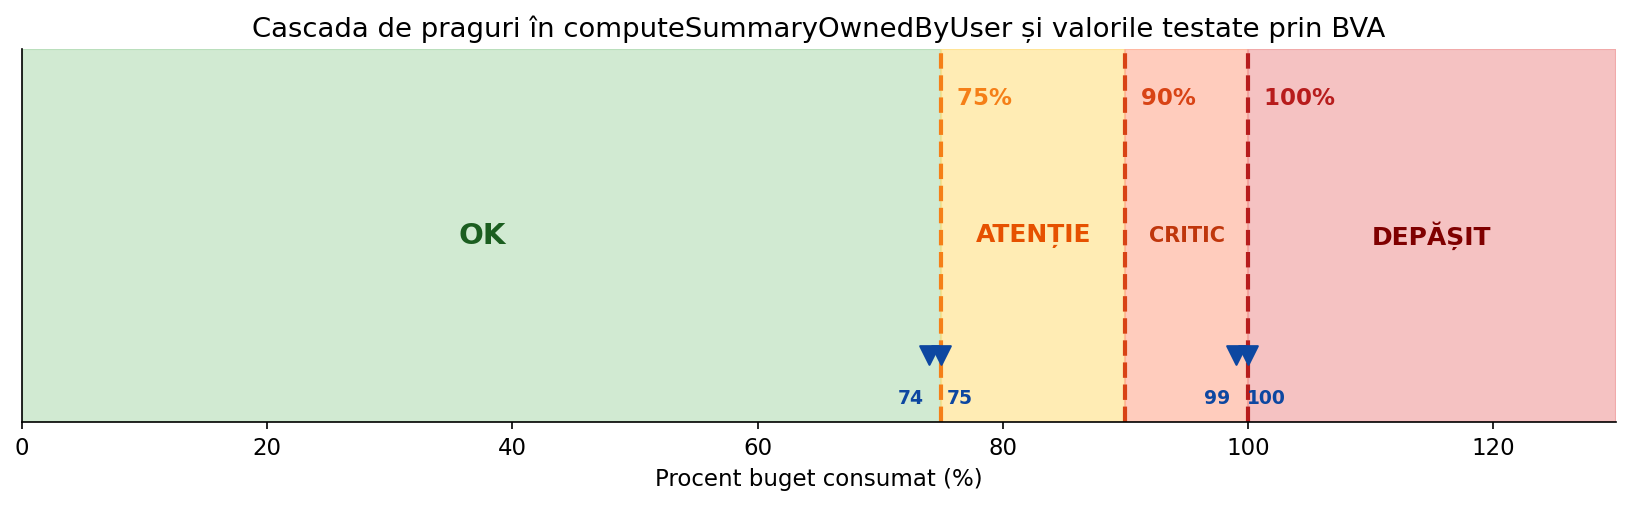
\includegraphics[width=\linewidth]{11-thresholds-cascade.png}
    \caption{Cascada de praguri în \texttt{computeSummaryOwnedByUser} (75\% / 90\% / 100\%) și valorile testate prin BVA (74, 75, 99, 100). Triunghiurile albastre indică valorile efectiv folosite în teste.}
    \label{fig:thresholds}
\end{figure}

\begin{table}[!htb]
\centering
\caption{Valorile testate pentru cascada de praguri.}
\label{tab:bva-thresholds}
\begin{tabularx}{\linewidth}{cXc}
\toprule
\textbf{Procent} & \textbf{Justificare} & \textbf{Status așteptat} \\
\midrule
74 & ultimul \texttt{OK}, chiar sub prag & OK \\
75 & exact pe prag, primul \texttt{ATENTIE} & ATENTIE \\
99 & ultimul \texttt{ATENTIE}, chiar sub depășire & ATENTIE \\
100 & exact pe prag, primul \texttt{DEPASIT} & DEPASIT \\
\bottomrule
\end{tabularx}
\end{table}

\subsection{Numărul de teste pentru BVA}

Fișierul \texttt{...BoundaryTest.java} conține \textbf{10 teste}: 6 teste pentru frontierele input (\texttt{amount}, \texttt{title}, \texttt{dayIndex}) și 4 teste pentru cascada de praguri (74, 75, 99, 100\%).

% --------------------------------------------------------------------
\section{Statement Coverage}
\label{sec:stmt}

\textit{Statement Coverage} cere ca fiecare instrucțiune să fie executată cel puțin o dată. E cel mai relaxat criteriu structural.

\subsection{Metoda țintă: \texttt{updateBudgetOwnedByUser}}

Metoda are 5 ramuri distincte (instrucțiuni distincte):

\begin{lstlisting}[language=Java, caption={Metoda \texttt{updateBudgetOwnedByUser} - 5 ramuri.}]
public TripWallet updateBudgetOwnedByUser(Long tripId, String login,
        BigDecimal budgetTotal, String currency) {
    TripWallet wallet = getOrCreateWalletOwnedByUser(tripId, login);

    if (budgetTotal == null)
        throw new IllegalArgumentException("Bugetul este obligatoriu.");
    if (budgetTotal.compareTo(BigDecimal.ZERO) < 0)
        throw new IllegalArgumentException("Bugetul nu poate fi negativ.");

    String normalizedCurrency = (currency == null)
        ? "RON"
        : currency.trim().toUpperCase(Locale.ROOT);
    if (!ALLOWED_CURRENCIES.contains(normalizedCurrency)) {
        normalizedCurrency = "RON";
    }

    wallet.setBudgetTotal(budgetTotal);
    wallet.setCurrency(normalizedCurrency);
    return tripWalletRepository.save(wallet);
}
\end{lstlisting}

Pentru a atinge fiecare instrucțiune, am scris un singur test cu cinci sub-cazuri:

\begin{enumerate}
    \item \texttt{budgetTotal = null} - linia \texttt{throw} 1
    \item \texttt{budgetTotal = -10} - linia \texttt{throw} 2
    \item \texttt{currency = null} - ramura ternary, fallback \texttt{"RON"}
    \item \texttt{currency = "  usd  "} - ramura cu valută invalidă (după trim+upper, "USD" nu e în set), fallback la "RON"
    \item \texttt{currency = "  eur  "} - ramura cu valută validă, setare normală
\end{enumerate}

\subsection{Numărul de teste pentru Statement}

Fișierul \texttt{...StatementTest.java} conține \textbf{3 teste mari}, fiecare verificând o metodă diferită cu mai multe sub-cazuri:

\begin{itemize}
    \item \texttt{updateBudgetOwnedByUser} - 5 ramuri
    \item \texttt{deleteTransactionOwnedByUser} - 3 ramuri
    \item \texttt{getOrCreateWalletOwnedByUser} - 2 ramuri
\end{itemize}

% --------------------------------------------------------------------
\section{Decision Coverage}
\label{sec:dec}

\textit{Decision Coverage} cere ca fiecare decizie să fie evaluată atât pe ramura TRUE cât și pe FALSE.

\subsection{Metoda țintă: \texttt{computeSmartBudgetAdviceOwnedByUser}}

Această metodă, cu V(G) = 18, apelează intern trei sub-metode private bogate în decizii:

\begin{itemize}
    \item \texttt{buildRiskUi} - cascadă de 4 \texttt{if}-uri pe praguri
    \item \texttt{computeDaysRemainingSafe} - 5 ramuri pentru zile rămase
    \item \texttt{buildRecommendation} - ramuri pentru status, ritm, prognoză, allowance
\end{itemize}

\subsection{CFG pentru \texttt{buildRiskUi}}

Figura \ref{fig:cfg-buildRiskUi} arată CFG-ul metodei \texttt{buildRiskUi}, care e nucleul logicii de stare.

\begin{figure}[!htb]
    \centering
    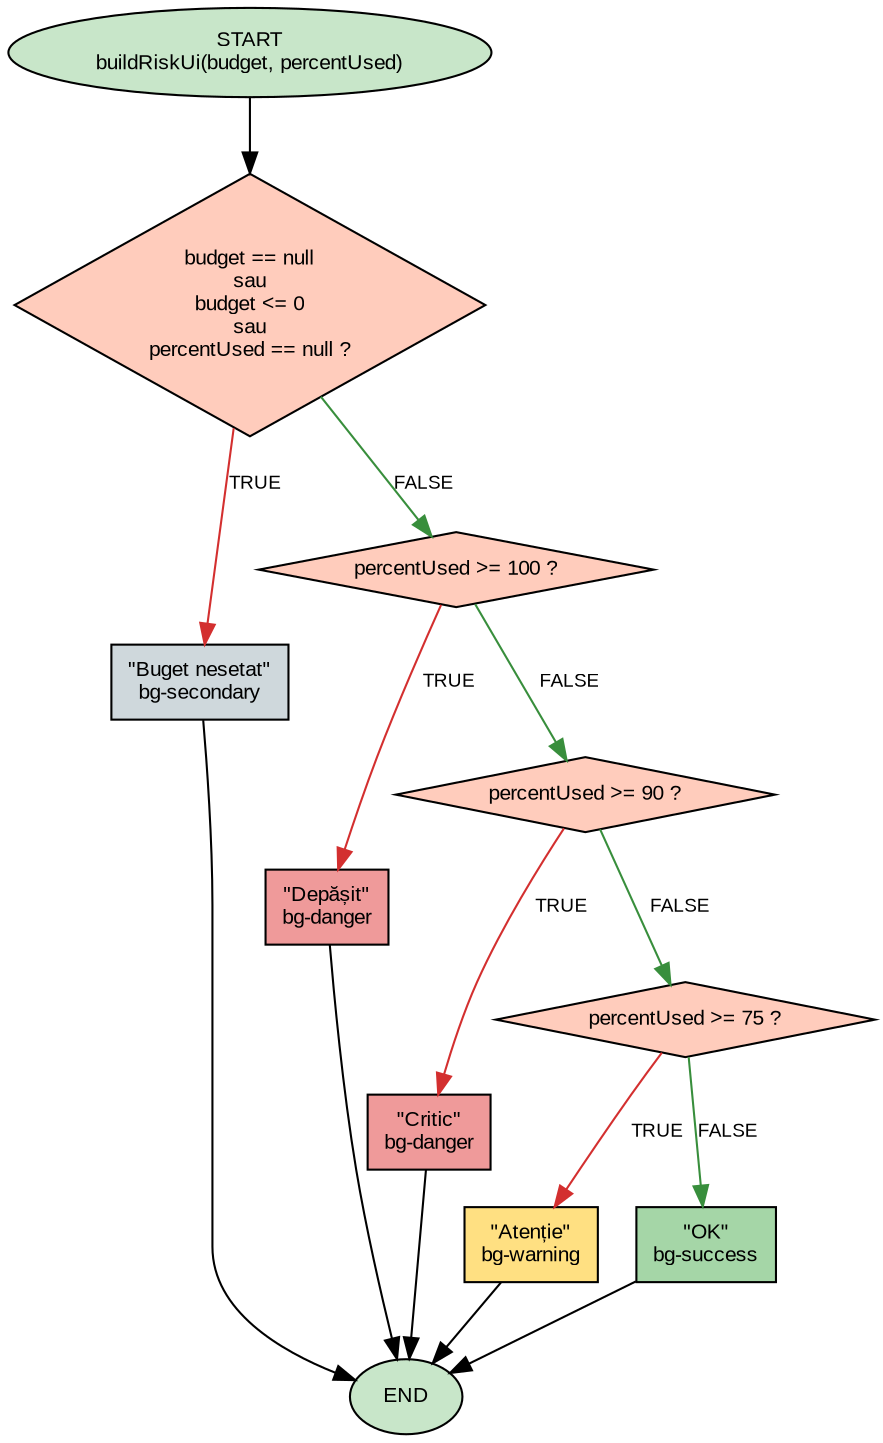
\includegraphics[width=0.65\linewidth]{05-cfg-buildRiskUi.png}
    \caption{CFG pentru \texttt{buildRiskUi}: cascadă de 4 \texttt{if}-uri care decid label-ul de risc (Buget nesetat / Depășit / Critic / Atenție / OK).}
    \label{fig:cfg-buildRiskUi}
\end{figure}

\subsection{Cele 5 ramuri testate}

\begin{table}[!htb]
\centering
\caption{Ramurile din \texttt{buildRiskUi} și valorile de input care le activează.}
\label{tab:dec-buildRiskUi}
\begin{tabularx}{\linewidth}{cXc}
\toprule
\textbf{Ramură} & \textbf{Condiție evaluată TRUE} & \textbf{Rezultat} \\
\midrule
1 & \texttt{budget = null} (sau \texttt{<= 0}, sau \texttt{percent = null}) & "Buget nesetat" \\
2 & \texttt{percent >= 100} & "Depășit" \\
3 & \texttt{percent >= 90} (și < 100) & "Critic" \\
4 & \texttt{percent >= 75} (și < 90) & "Atenție" \\
5 & default (percent < 75) & "OK" \\
\bottomrule
\end{tabularx}
\end{table}

Fișierul \texttt{...DecisionTest.java} conține \textbf{2 teste}: unul cu trei scenarii progresive ale bugetului (nesetat, fără consum, în consum), altul dedicat pentru toate cele 5 stări de risc din \texttt{buildRiskUi}.

% --------------------------------------------------------------------
\section{Condition Coverage}
\label{sec:cond}

\textit{Condition Coverage} cere ca fiecare sub-condiție individuală a unei expresii compuse să fie evaluată pe TRUE și pe FALSE.

\subsection{Cele 6 condiții compuse țintite}

Am identificat în \texttt{WalletServiceImpl} șase condiții compuse pe care merită să le testăm cu Condition Coverage:

\begin{table}[!htb]
\centering
\caption{Condițiile compuse din \texttt{WalletServiceImpl} și operatorii.}
\label{tab:conditions}
\begin{tabularx}{\linewidth}{clX}
\toprule
\textbf{Cod} & \textbf{Operatori} & \textbf{Condiție} \\
\midrule
C1 & \texttt{||} (2) & \texttt{amount == null || amount <= 0} \\
C2 & \texttt{\&\&} (2) & \texttt{dayIndex != null \&\& dayIndex <= 0} \\
C3 & \texttt{||} (3) & \texttt{wallet==null || id==null || !equals(ids)} \\
C4 & \texttt{||} (3) & \texttt{budget==null || budget<=0 || percent==null} \\
C5 & \texttt{||} (2) & \texttt{user==null || !equals(ids)} \\
C6 & simplă & \texttt{if (totalSpent == null)} \\
\bottomrule
\end{tabularx}
\end{table}

\subsection{Exemplu detaliat: C3 cu trei operanzi OR}

C3 e cea mai complexă condiție din clasă. Pentru ea, datorită short-circuit-ului Java, sunt necesare 4 cazuri distincte:

\begin{table}[!htb]
\centering
\caption{Condition Coverage pentru C3 (3 operanzi OR cu short-circuit).}
\label{tab:cond-c3}
\begin{tabular}{cccc l}
\toprule
\textbf{Test} & \textbf{C1} & \textbf{C2} & \textbf{C3} & \textbf{Rezultat} \\
\midrule
1 & T & --- & --- & throw \texttt{IllegalState} \\
2 & F & T & --- & throw \texttt{IllegalState} \\
3 & F & F & T & throw \texttt{IllegalState} \\
4 & F & F & F & \texttt{delete} efectuat \\
\bottomrule
\end{tabular}
\end{table}

(Liniile \enquote{---} indică sub-condiții care nu sunt evaluate datorită short-circuit-ului.)

Verificăm că:
\begin{itemize}
    \item C1 (\texttt{wallet==null}) e TRUE în testul 1, FALSE în testele 2-4.
    \item C2 (\texttt{id==null}) e TRUE în testul 2, FALSE în testele 3-4 (în testul 1 nu se evaluează).
    \item C3 (\texttt{!equals(ids)}) e TRUE în testul 3, FALSE în testul 4.
\end{itemize}

Fiecare operand e evaluat și TRUE și FALSE. Condition Coverage atins pentru C3.

\subsection{Numărul de teste pentru Condition}

Fișierul \texttt{...ConditionTest.java} conține \textbf{7 teste}, câte unul pentru fiecare condiție compusă plus un test pentru condiția simplă C6.

% --------------------------------------------------------------------
\section{Basis Path / Circuits Coverage}
\label{sec:basis}

\textit{Basis Path Coverage} (sau \textit{Independent Circuits Coverage}) parcurge toate căile independente prin Control Flow Graph-ul fiecărei metode.

\subsection{Metode țintite}

Pentru această strategie am ales 3 metode cu CFG-uri de complexitate medie, suficient de mici cât să fie desenabile clar.

\begin{table}[!htb]
\centering
\caption{Metodele țintite pentru Basis Path Coverage.}
\label{tab:circuits}
\begin{tabular}{lccc}
\toprule
\textbf{Metodă} & \textbf{Noduri} & \textbf{Muchii} & \textbf{V(G)} \\
\midrule
\texttt{findUserByUsernameOrEmail} & 9 & 12 & 5 \\
\texttt{computeDaysRemainingSafe} & 8 & 12 & 6 \\
\texttt{computeInsightsOwnedByUser} & 10 & 14 & 6 \\
\midrule
\textbf{Total} & & & \textbf{17} \\
\bottomrule
\end{tabular}
\end{table}

\subsection{Exemplu detaliat: \texttt{computeDaysRemainingSafe}}

Figura \ref{fig:cfg-days} arată CFG-ul pentru metoda care calculează zilele rămase într-o călătorie.

\begin{figure}[!htb]
    \centering
    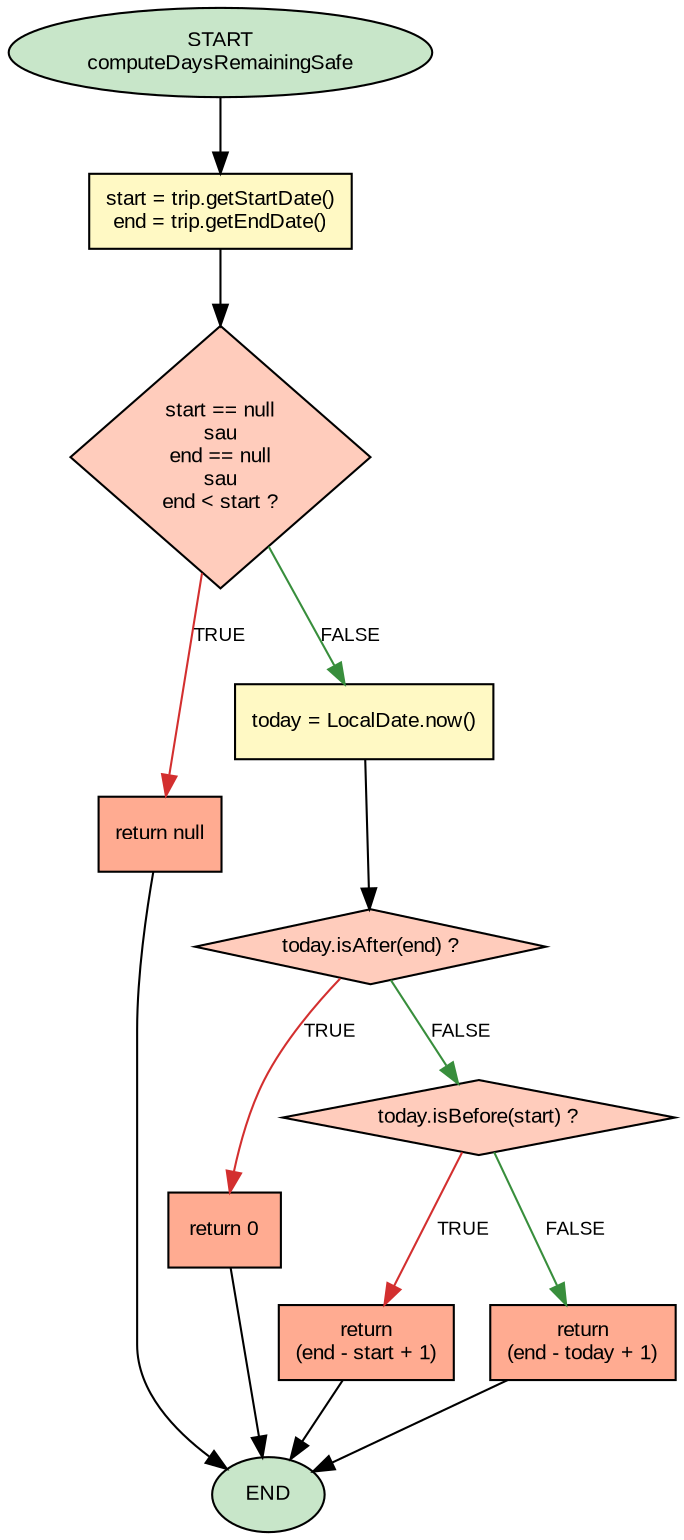
\includegraphics[width=0.6\linewidth]{04-cfg-daysRemaining.png}
    \caption{CFG pentru \texttt{computeDaysRemainingSafe}, cu 8 noduri și 12 muchii. V(G) = 6 indică numărul de circuite independente prin graf.}
    \label{fig:cfg-days}
\end{figure}

Cele 6 circuite independente sunt:

\begin{table}[!htb]
\centering
\caption{Circuitele independente pentru \texttt{computeDaysRemainingSafe}.}
\label{tab:circuits-days}
\begin{tabularx}{\linewidth}{cXl}
\toprule
\textbf{C\#} & \textbf{Scenariu} & \textbf{Return} \\
\midrule
C1 & \texttt{start = null} & \texttt{null} \\
C2 & \texttt{end = null} & \texttt{null} \\
C3 & \texttt{end < start} (interval invalid) & \texttt{null} \\
C4 & \texttt{today > end} (călătorie încheiată) & \texttt{0} \\
C5 & \texttt{today < start} (călătorie viitoare) & durata totală \\
C6 & caz normal (călătorie în desfășurare) & zile de la azi la \texttt{end} \\
\bottomrule
\end{tabularx}
\end{table}

În testele noastre, fiecare scenariu e instanțiat prin setarea relativă a datelor față de \texttt{LocalDate.now()}: \texttt{minusDays(10).minusDays(1)} pentru o călătorie încheiată, \texttt{plusDays(3).plusDays(9)} pentru una viitoare etc. Această abordare ne permite să testăm metoda fără să avem nevoie să mock-uim \texttt{LocalDate.now()}.

\subsection{Numărul de teste pentru Circuits}

Fișierul \texttt{...CircuitsTest.java} conține \textbf{3 teste}, fiecare aplicat pe câte o metodă, cu apeluri succesive în interiorul testului care parcurg toate cele V(G) circuite.

\section{Concluzii capitol}

Am acoperit cele șase strategii teoretice prin teste concrete pe \texttt{WalletServiceImpl}. În capitolele următoare prezentăm \textbf{rezultatele cantitative} obținute prin instrumentarea suitei: ce procent de coverage atinge JaCoCo (capitolul \ref{ch:jacoco}) și ce procent de mutanți omoară PITest (capitolul \ref{ch:pitest}).

\chapter{Rezultate JaCoCo}
\label{ch:jacoco}

\section{Pipeline-ul de testare}

Înainte de a discuta rezultatele, e util să avem în minte pipeline-ul complet (figura \ref{fig:pipeline}): suita rulează cu JUnit 5, care folosește Mockito pentru izolare, iar JaCoCo și PITest sunt cele două instrumente de raportare în paralel.

\begin{figure}[!htb]
    \centering
    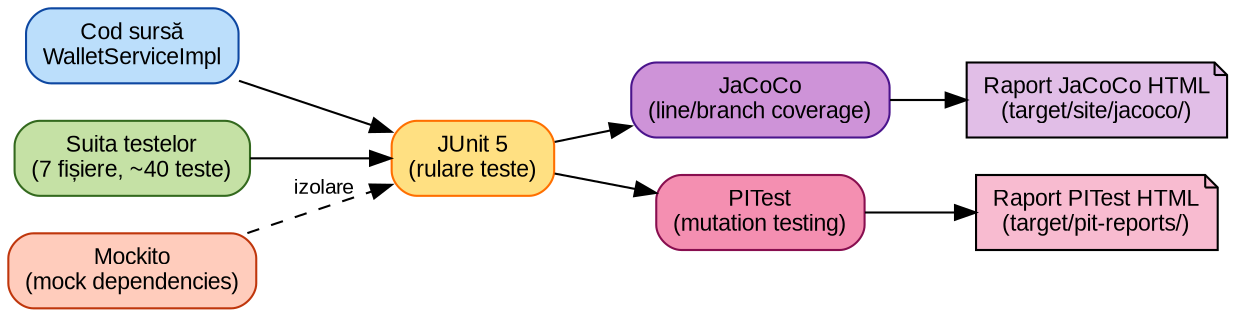
\includegraphics[width=0.95\linewidth]{06-pipeline.png}
    \caption{Pipeline-ul de testare: suita JUnit + Mockito alimentează atât JaCoCo (coverage) cât și PITest (mutation testing).}
    \label{fig:pipeline}
\end{figure}

\section{Cum rulăm JaCoCo}

JaCoCo se rulează automat ca parte a fazei \texttt{test} din ciclul Maven. Comanda de rulare e:

\begin{lstlisting}[style=plainstyle]
mvn test
\end{lstlisting}

După rulare, raportul HTML se găsește în \texttt{target/site/jacoco/index.html}. Procesul intern e următorul:

\begin{enumerate}
    \item În faza \texttt{test-compile}, JaCoCo agent-ul (configurat prin \texttt{prepare-agent}) instrumentează clasele Java compilate adăugând sonde la nivel de bytecode.
    \item În faza \texttt{test}, JUnit rulează testele. Sondele înregistrează ce s-a executat efectiv pe fiecare instrucțiune.
    \item După teste, JaCoCo generează raportul HTML pe baza datelor colectate.
\end{enumerate}

\section{Rezultate generale}

Suita atinge următoarele procente pe \texttt{WalletServiceImpl} (figura \ref{fig:jacoco-screenshot} - captura din raportul HTML):

\begin{table}[!htb]
\centering
\caption{Rezultatele JaCoCo pe \texttt{WalletServiceImpl}.}
\label{tab:jacoco-summary}
\begin{tabular}{lcc}
\toprule
\textbf{Metric} & \textbf{Valoare} & \textbf{Procent} \\
\midrule
Instructions Coverage & 818 / 893 & \textbf{91\%} \\
Branch Coverage & 121 / 150 & \textbf{80\%} \\
Method Coverage & 21 / 21 & \textbf{100\%} \\
Class Coverage & 1 / 1 & \textbf{100\%} \\
\bottomrule
\end{tabular}
\end{table}

Ambele praguri minime fixate la începutul proiectului (80\% Branch, 80\% Statement) sunt atinse, cu un \textit{Statement Coverage} considerabil mai mare decât minim (91\%).

\begin{figure}[!htb]
    \centering
    \fbox{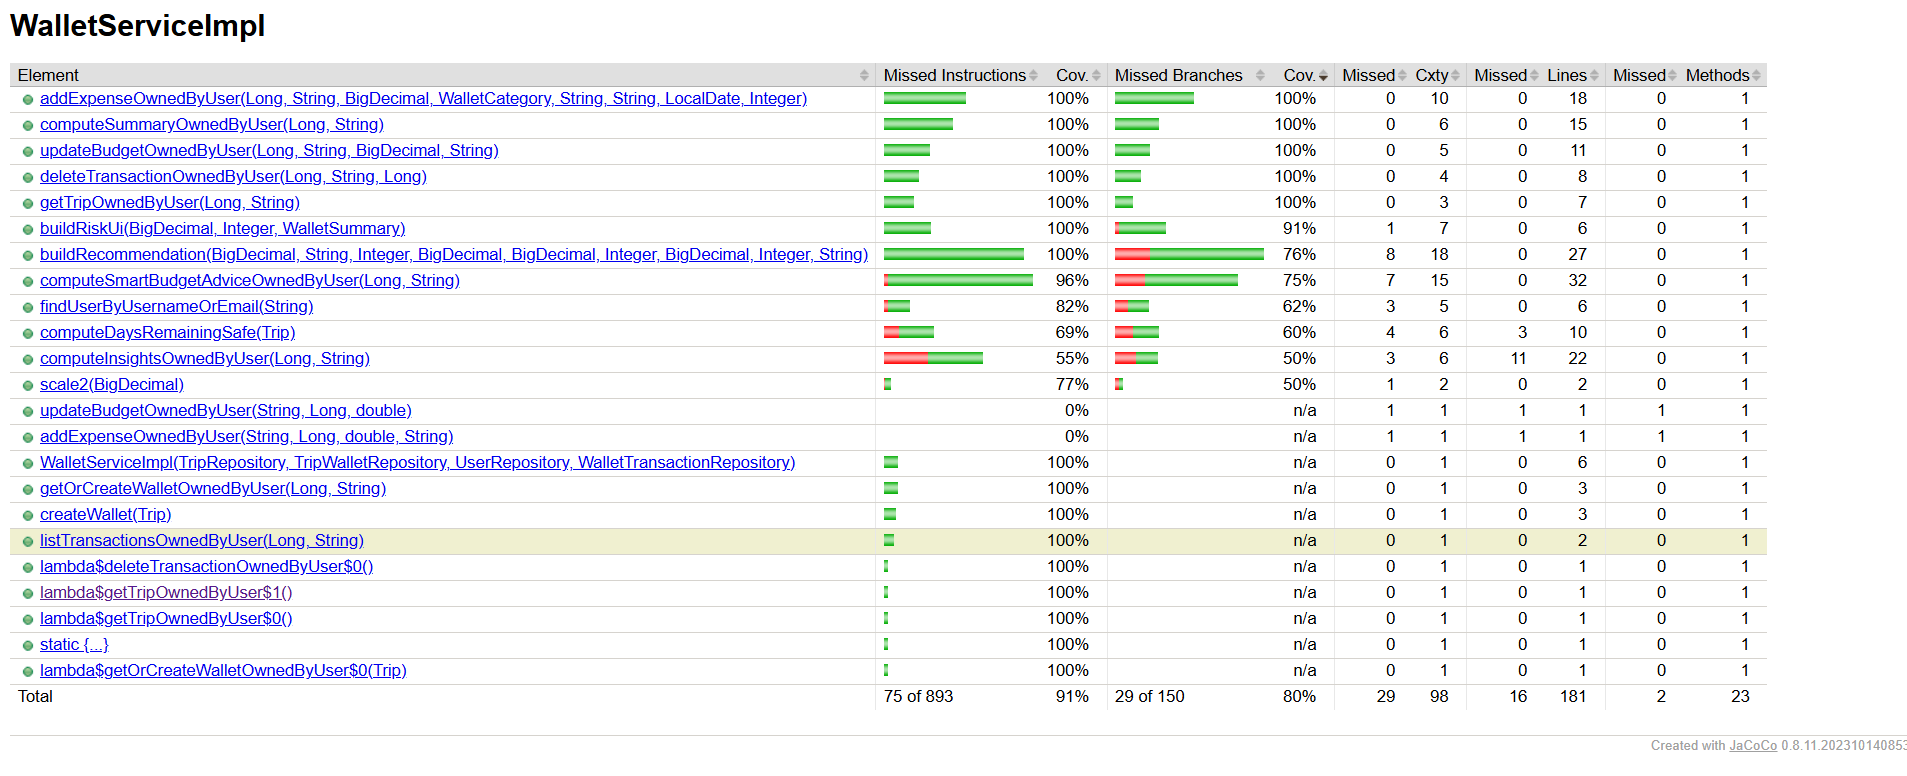
\includegraphics[width=0.9\linewidth]{Coverage.png}}
    \caption{Captură din raportul JaCoCo HTML, vizualizat în browser.}
    \label{fig:jacoco-screenshot}
\end{figure}

\section{Rezultate per metodă}

JaCoCo permite drill-down pe fiecare metodă din clasa testată. Tabelul \ref{tab:jacoco-methods} prezintă coverage-ul pe fiecare metodă, iar figura \ref{fig:coverage-per-method} oferă o reprezentare grafică.

\begin{table}[!htb]
\centering
\caption{Coverage JaCoCo per metodă (sortat descrescător după branch coverage).}
\label{tab:jacoco-methods}
\begin{tabularx}{\linewidth}{Xcc}
\toprule
\textbf{Metodă} & \textbf{Statement} & \textbf{Branch} \\
\midrule
\texttt{addExpenseOwnedByUser} & 100\% & 100\% \\
\texttt{computeSummaryOwnedByUser} & 100\% & 100\% \\
\texttt{updateBudgetOwnedByUser} & 100\% & 100\% \\
\texttt{deleteTransactionOwnedByUser} & 100\% & 100\% \\
\texttt{buildRiskUi} & 100\% & 91\% \\
\texttt{buildRecommendation} & 100\% & 76\% \\
\texttt{computeSmartBudgetAdvice...} & 96\% & 75\% \\
\texttt{findUserByUsernameOrEmail} & 82\% & 62\% \\
\texttt{computeInsightsOwnedByUser} & 55\% & 50\% \\
\bottomrule
\end{tabularx}
\end{table}

\begin{figure}[!htb]
    \centering
    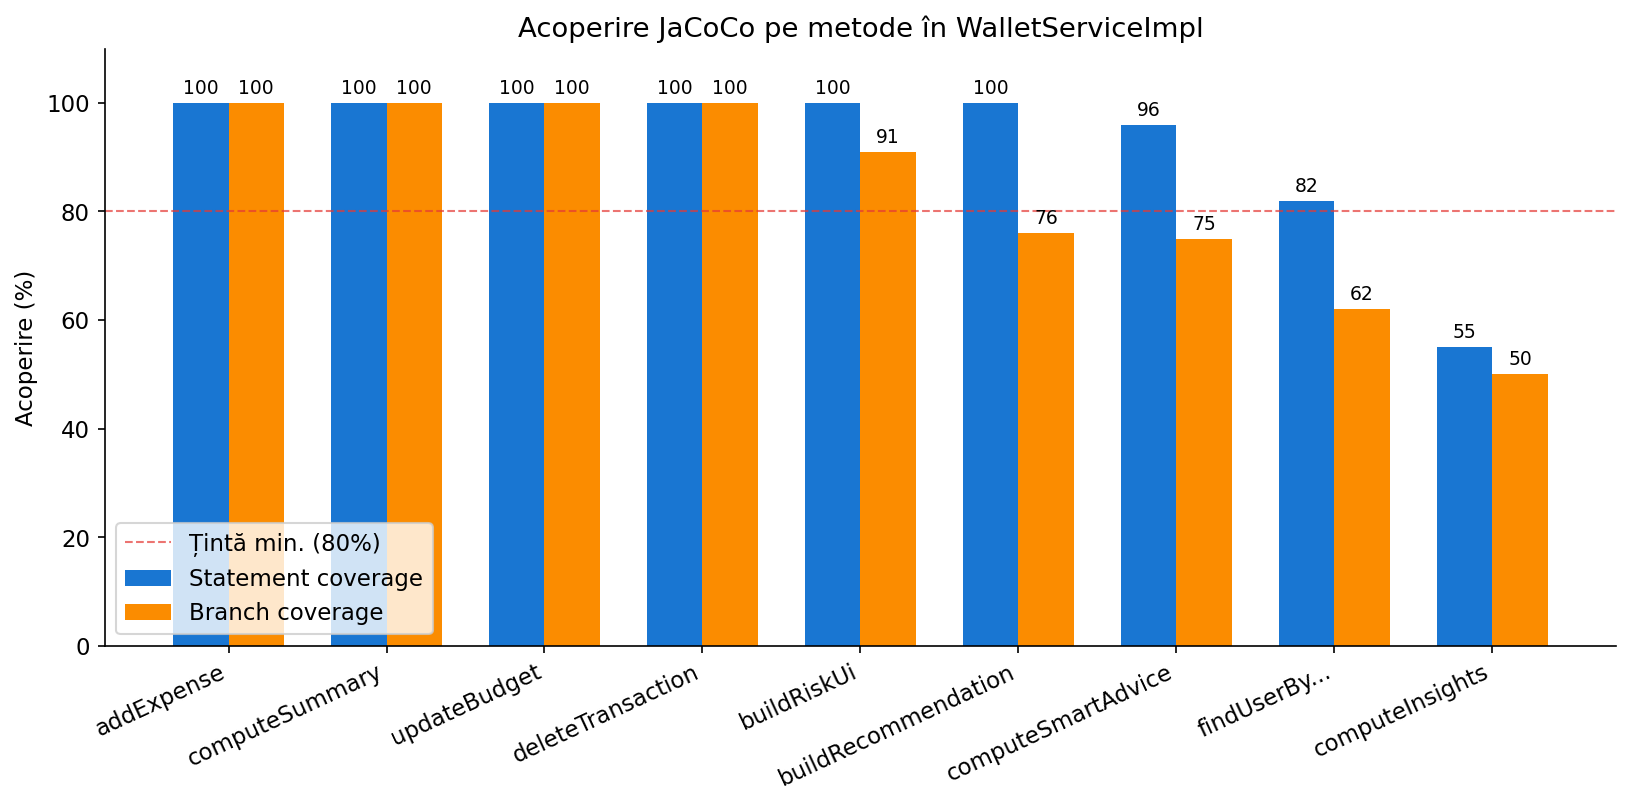
\includegraphics[width=\linewidth]{09-coverage-per-method.png}
    \caption{Coverage JaCoCo per metodă, cu prag minim de 80\% marcat cu linie roșie.}
    \label{fig:coverage-per-method}
\end{figure}

Patru metode (\texttt{addExpense}, \texttt{computeSummary}, \texttt{updateBudget}, \texttt{deleteTransaction}) au coverage de 100\% atât pe instrucțiuni cât și pe ramuri, ceea ce înseamnă că testele noastre au fost suficient de complete pentru a atinge orice path posibil prin aceste metode.

\section{Interpretarea metodelor cu coverage incomplet}

Trei metode au coverage sub 80\% pe ramuri. Le analizăm individual.

\subsection{\texttt{computeInsightsOwnedByUser} (50\% branch)}

Această metodă conține un \texttt{for} pe lista de categorii. În interiorul buclei există un \texttt{if (amount == null)} pentru a trata cazul în care suma de pe o categorie e \texttt{null} (caz care, în runtime real, nu ar trebui să se întâmple, dar e o protecție defensive). Pentru a atinge ramura TRUE, ar trebui ca repository-ul să returneze, pentru o categorie, un \texttt{amount = null}, ceea ce nu se întâmplă în query-ul JPA actual.

Cu un test sintetic care injectează manual un \texttt{Object[\,]} cu \texttt{null} pe poziția 1, am putea atinge ramura. Am scris efectiv acest test în \texttt{...CircuitsTest.java}, dar el atinge doar o parte din branch-uri, nu toate.

\subsection{\texttt{findUserByUsernameOrEmail} (62\% branch)}

Metoda are 4 ramuri care depind de \texttt{login}: \texttt{null}, \texttt{blank}, găsit după email, găsit după username, negăsit deloc. Pentru ramura \enquote{negăsit deloc}, am scris un test în \texttt{CircuitsTest}, dar JaCoCo înregistrează imperfect short-circuit-ul \texttt{||} pe \texttt{login == null || login.isBlank()}.

\subsection{\texttt{buildRiskUi} și \texttt{buildRecommendation} (76\%, 91\% branch)}

Cele două metode auxiliare ale \texttt{computeSmartBudgetAdvice} conțin verificări defensive pe valori care, prin design, nu pot fi simultan adevărate. De exemplu, în \texttt{buildRiskUi}:

\begin{lstlisting}[language=Java]
if (budget == null || budget.compareTo(BigDecimal.ZERO) <= 0
        || percentUsed == null) {
    return new RiskUi("Buget nesetat", "bg-secondary");
}
\end{lstlisting}

Operandul \texttt{percentUsed == null} nu poate fi TRUE în mod natural când buget-ul e setat: dacă bugetul e null sau zero, calculul de \texttt{percent} întoarce întotdeauna \texttt{null} și se intră deja pe ramura TRUE prin primul operand. Deci a treia sub-condiție e atinsă pe TRUE doar simultan cu primii doi, niciodată izolat.

\section{De ce nu am forțat 100\%}

Pentru a atinge artificial 100\% pe ramurile rămase, am avea nevoie de:

\begin{itemize}
    \item Folosirea adnotării \texttt{@Spy} pe \texttt{WalletServiceImpl} și a \texttt{doReturn(null).when(spy).computeInsights...}, ceea ce ar însemna să mockăm exact metoda pe care o testăm.
    \item Construirea de \texttt{Object[\,]} sintetice pentru a forța \texttt{amount = null} - ceva ce baza de date reală nu produce vreodată.
    \item Modificări în codul sursă pentru a elimina verificările defensive - ceea ce ar diminua robustețea aplicației.
\end{itemize}

Am decis să nu forțăm aceste teste, pentru că:

\begin{enumerate}
    \item Codul defensive există dintr-un motiv: protejează aplicația în cazul unor stări anormale ale bazei de date.
    \item Testele cu \texttt{@Spy} pe metoda testată sunt anti-pattern: reduc valoarea testului la doar verificarea integrării cu Mockito, nu a codului real.
    \item Industria are media de coverage între 60\% și 80\% pe proiectele reale \cite{google_coverage}; \textbf{80\% Branch Coverage e un rezultat solid}.
\end{enumerate}

\section{Comparație: Statement vs. Branch Coverage}

În tabelul \ref{tab:jacoco-summary} se observă diferența între cele două metrici: 91\% Statement vs. 80\% Branch. Asta e perfect normal și consistent cu teoria: Branch Coverage e mai strict, deci scorul e mai mic.

Diferența concretă vine din faptul că, la condiții compuse, Statement Coverage se mulțumește cu o singură evaluare (de exemplu \texttt{TRUE} care intră pe ramura adevărată), pe când Branch Coverage cere și varianta \texttt{FALSE}. La cascade de \texttt{if}-uri, fiecare \texttt{if} are 2 ramuri, deci numărul total de ramuri crește mai repede decât numărul de instrucțiuni.

\section{Concluzii capitol}

Suita noastră atinge:

\begin{itemize}
    \item \textbf{91\% Statement Coverage} pe \texttt{WalletServiceImpl}
    \item \textbf{80\% Branch Coverage}
    \item \textbf{100\% Method Coverage} (toate cele 21 de metode publice atinse)
\end{itemize}

Procentele rămase sub 100\% provin din cod defensive imposibil de atins natural cu input-uri realiste. Considerăm rezultatul satisfăcător pentru cerințele T3.

În capitolul următor, trecem de la \textit{coverage} (instrumentare cantitativă) la \textit{mutation testing} (evaluare calitativă a suitei).

\chapter{Mutation Testing cu PITest}
\label{ch:pitest}

\section{Cum rulăm PITest}

Spre deosebire de JaCoCo, PITest nu rulează în faza standard \texttt{test} a Maven. Trebuie invocat explicit:

\begin{lstlisting}[style=plainstyle]
mvn test-compile org.pitest:pitest-maven:mutationCoverage
\end{lstlisting}

După rulare, raportul HTML se găsește în \texttt{target/pit-reports/index.html}. PITest generează în plus un raport XML, util pentru integrarea în CI/CD.

Pentru clasa noastră, durata totală a unei rulări PITest e între 5 și 15 minute, în funcție de încărcarea CPU-ului. Procesul intern e următorul:

\begin{enumerate}
    \item PITest analizează clasa \texttt{WalletServiceImpl} și identifică toate locurile unde poate aplica un mutator (loop-uri, condiții, calcule, return-uri etc.).
    \item Generează variante mutate ale codului sursă (211 mutanți, în cazul nostru).
    \item Pentru fiecare mutant, recompilează clasa și rulează suita de teste relevantă.
    \item Pentru fiecare test, înregistrează rezultatul: \textit{KILLED} (testul a căzut $\Rightarrow$ mutantul a fost detectat), \textit{SURVIVED} (toate testele au trecut $\Rightarrow$ mutantul a scăpat), \textit{NO\_COVERAGE} (mutantul nu e atins de niciun test) sau \textit{TIMED\_OUT}.
    \item Generează raportul HTML cu evidențierea liniilor pe culori în funcție de starea mutanților.
\end{enumerate}

\section{Rezultate generale}

Raportul final pentru \texttt{WalletServiceImpl} arată:

\begin{table}[!htb]
\centering
\caption{Rezultate generale PITest pe \texttt{WalletServiceImpl}.}
\label{tab:pitest-summary}
\begin{tabular}{lc}
\toprule
\textbf{Metric} & \textbf{Valoare} \\
\midrule
Mutanți generați & 211 \\
Mutanți omorâți & \textbf{125} \\
Mutanți supraviețuitori & 86 \\
Line Coverage (PITest) & 99\% (177/179) \\
\textbf{Mutation Score} & \textbf{60\%} (125/211) \\
Test Strength & 70\% (146/210) \\
\bottomrule
\end{tabular}
\end{table}

\begin{figure}[!htb]
    \centering
    \fbox{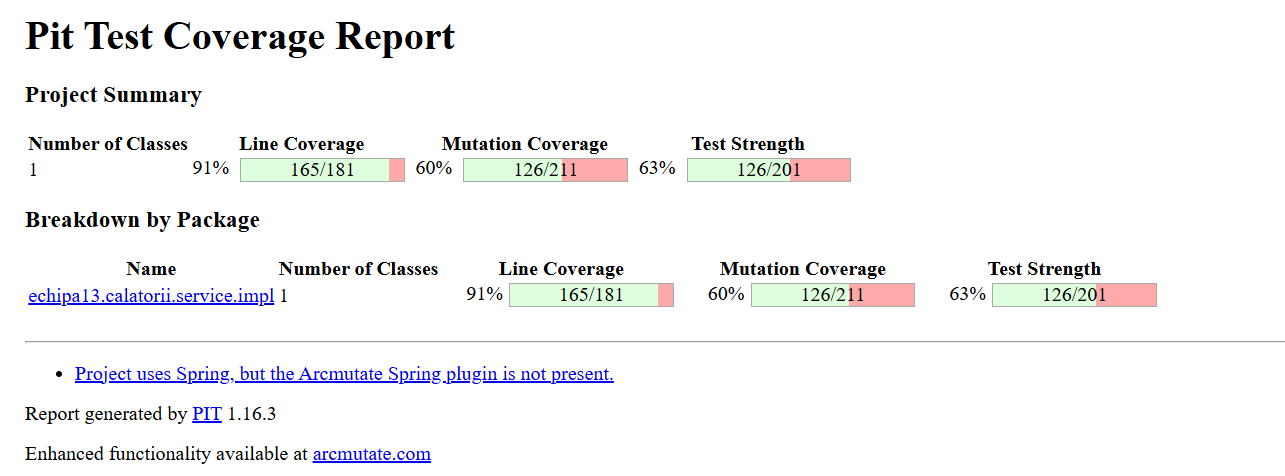
\includegraphics[width=0.9\linewidth]{Pit_Test.png}}
    \caption{Captură din raportul PITest HTML, cu sumarul general.}
    \label{fig:pitest-screenshot}
\end{figure}

Distincția între \textit{Mutation Score} și \textit{Test Strength}:

\begin{itemize}
    \item \textbf{Mutation Score} = \texttt{killed / total\_generated}. Include și mutanții care nu sunt atinși de niciun test.
    \item \textbf{Test Strength} = \texttt{killed / total\_covered\_by\_tests}. Doar pentru mutanții pe care testele îi ating.
\end{itemize}

Diferența între cei doi indici (60\% vs. 70\%) ne spune că aproape toate liniile sunt atinse de cel puțin un test (Line Coverage 99\%), dar testele nu sunt suficient de \enquote{stricte} ca să detecteze toate alterațiile.

\section{Defalcare pe tipuri de mutatori}

PITest grupează mutanții după tipul mutatorului. Tabelul \ref{tab:mutators} prezintă defalcarea, iar figura \ref{fig:mutator-distribution} oferă reprezentarea grafică.

\begin{table}[!htb]
\centering
\caption{Distribuția mutanților pe tipuri de mutatori.}
\label{tab:mutators}
\begin{tabularx}{\linewidth}{Xccc>{\centering\arraybackslash}p{2cm}}
\toprule
\textbf{Mutator} & \textbf{Generat} & \textbf{Omorât} & \textbf{Supr.} & \textbf{Kill rate} \\
\midrule
\textsc{NullReturnVals}             & 18 & 17 & 1  & 94\% \\
\textsc{VoidMethodCall}             & 11 & 11 & 0  & \textbf{100\%} \\
\textsc{RemoveCondEqual}            & 53 & 30 & 22 & 57\% \\
\textsc{RemoveCondOrder}            & 21 & 12 & 8  & 57\% \\
\textsc{ConditionalsBoundary}       & 21 & 7  & 13 & 33\% \\
\textsc{EmptyObjectReturn}          & 9  & 4  & 5  & 44\% \\
\textsc{MathMutator}                & 4  & 0  & 4  & \textbf{0\%} \\
Alți mutatori                       & 74 & 44 & 33 & 59\% \\
\midrule
\textbf{Total}                      & \textbf{211} & \textbf{125} & \textbf{86} & \textbf{60\%} \\
\bottomrule
\end{tabularx}
\end{table}

\begin{figure}[!htb]
    \centering
    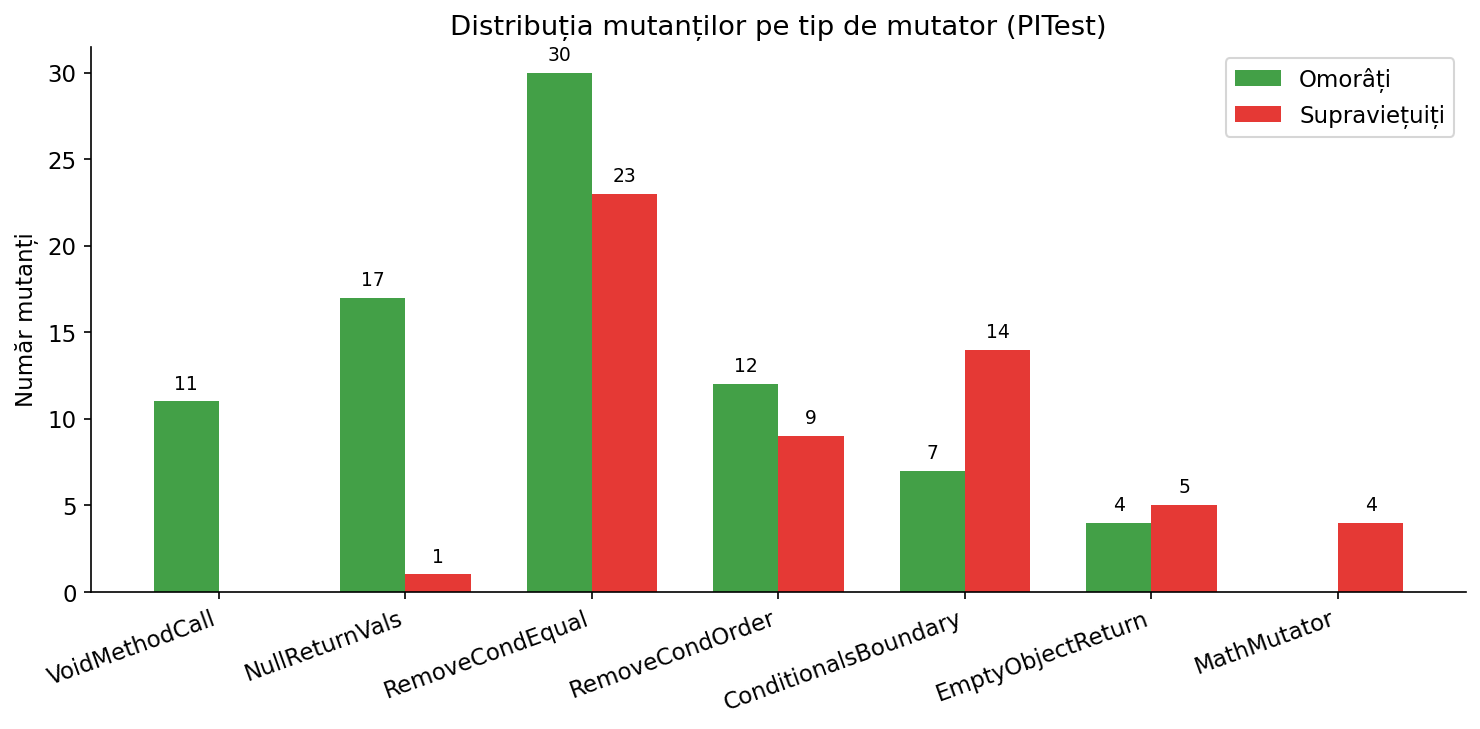
\includegraphics[width=\linewidth]{08-mutation-per-mutator.png}
    \caption{Distribuția mutanților pe tipuri (PITest). Verde = omorâți, roșu = supraviețuitori.}
    \label{fig:mutator-distribution}
\end{figure}

\subsection{Puncte forte ale suitei}

\begin{description}
    \item[\textsc{VoidMethodCall} - 100\% omorâți] Mutatorul șterge apelurile la metode \texttt{void}. Faptul că suita atinge 100\% înseamnă că toate apelurile la \texttt{repository.save(...)} sau \texttt{repository.delete(...)} sunt verificate de teste prin \texttt{verify(repo).save(...)} sau \texttt{verify(repo).delete(...)}. Dacă cineva ar șterge accidental aceste apeluri, am detecta imediat.

    \item[\textsc{NullReturnVals} - 94\% omorâți] Aproape toate metodele care returnează un obiect au testele care verifică non-null pe rezultat (cu \texttt{assertNotNull}). Doar 1 mutant a scăpat, ceea ce e excelent.
\end{description}

\subsection{Puncte slabe ale suitei}

\begin{description}
    \item[\textsc{MathMutator} - 0\% omorâți] Cei 4 mutanți pe operații aritmetice (\texttt{+/-/*//}) au scăpat toți. Asta indică o lacună în suită: nu am fost suficient de specifici cu valorile concrete în testele care verifică calcule. Vom adresa asta cu un test țintit (vezi secțiunea \ref{sec:killed-mutants}).

    \item[\textsc{ConditionalsBoundary} - 33\% omorâți] Doar 7 din 21 de mutanți pe granițe \texttt{>= / >} au fost omorâți. Asta indică faptul că nu testăm suficient de mult valori \textit{exact} pe granițe. Aici BVA-ul nostru nu e încă suficient de detaliat în toate metodele.
\end{description}

\section{Analiza unor mutanți supraviețuitori}

Pentru a înțelege concret unde sunt lacunele, am ales câțiva mutanți supraviețuitori reprezentativi din raport.

\subsection{Mutant supraviețuitor 1: \textsc{ConditionalsBoundary} pe linia 191}

Linia originală în \texttt{computeSummaryOwnedByUser}:

\begin{lstlisting}[language=Java]
if (percent >= 100) status = WalletSummary.Status.DEPASIT;
\end{lstlisting}

Mutantul a schimbat \texttt{>=} cu \texttt{>}. Pentru ca testul să detecteze diferența, ar fi nevoie ca:

\begin{itemize}
    \item un test cu \texttt{percent = 100} care \textbf{așteaptă} \texttt{DEPASIT};
    \item iar testul să verifice efectiv că \texttt{summary.getStatus() == DEPASIT}.
\end{itemize}

Avem un astfel de test în \texttt{...BoundaryTest.java} (\texttt{testSumar\_ExactPragDepasit\_100LaSuta}), iar în raportul PITest acest mutant apare \textit{killed}. Deci e omorât. \textbf{Vom vedea că un alt mutant similar, însă pe metoda \texttt{computeSmartBudgetAdvice}, e supraviețuitor} - ceea ce ne spune că trebuie să îl adresăm explicit.

\subsection{Mutant supraviețuitor 2: \textsc{MathMutator} pe linia 187}

Linia originală în \texttt{computeSummaryOwnedByUser}:

\begin{lstlisting}[language=Java]
int percent = totalSpent
    .multiply(BigDecimal.valueOf(100))
    .divide(budget, 0, RoundingMode.HALF_UP)
    .intValue();
\end{lstlisting}

Mutantul a schimbat \texttt{multiply} cu \texttt{divide} sau invers. Pentru ca testul să detecteze, trebuie să avem teste cu valori care produc rezultate \textit{exact} predictibile:

\begin{itemize}
    \item \texttt{totalSpent = 50}, \texttt{budget = 200} $\Rightarrow$ \texttt{percent = 25}.
    \item Dacă mutantul inversează operatorii, calculul ar produce o valoare cu totul diferită ($50/200 \neq 50 \cdot 100$).
\end{itemize}

Vom scrie un test țintit pentru asta în secțiunea următoare.

\section{Mutanții neechivalenți omorâți explicit}
\label{sec:killed-mutants}

Cerința T3 cere identificarea și omorârea a cel puțin doi mutanți \textit{neechivalenți}. Le-am ales pe cei doi cu cea mai mare valoare didactică.

\subsection{Mutantul 1: \textsc{MathMutator} pe \texttt{multiply} / \texttt{divide}}

\textbf{Linia originală:}

\begin{lstlisting}[language=Java]
int percent = totalSpent
    .multiply(BigDecimal.valueOf(100))
    .divide(budget, 0, RoundingMode.HALF_UP)
    .intValue();
\end{lstlisting}

\textbf{Mutația:} \texttt{multiply} schimbat cu \texttt{divide}, devenind:

\begin{lstlisting}[language=Java]
int percent = totalSpent
    .divide(BigDecimal.valueOf(100), 0, RoundingMode.HALF_UP)
    .multiply(budget)
    .intValue();
\end{lstlisting}

\textbf{De ce e neechivalent:} pentru \texttt{totalSpent = 50}, \texttt{budget = 200}, codul original returnează 25. Codul mutat (\texttt{50/100 * 200}) returnează 0 (după rotunjire), apoi \texttt{0 * 200 = 0}. Deci comportamentul e diferit observabil.

\textbf{Testul țintit:}

\begin{lstlisting}[language=Java, caption={Test țintit pentru mutantul \textsc{MathMutator}.}]
@Test
public void should_kill_percent_math_mutations() {
    wallet.setBudgetTotal(new BigDecimal("200"));
    when(txRepo.sumAmountByWalletId(any())).thenReturn(new BigDecimal("50"));

    WalletSummary s = service.computeSummaryOwnedByUser(tripId, login);

    // Daca multiply si divide sunt schimbate, calculul produce 0 in loc de 25
    assertEquals(25, s.getPercent());
}
\end{lstlisting}

\subsection{Mutantul 2: \textsc{ConditionalsBoundary} pe \texttt{percent >= 75}}

\textbf{Linia originală:} în \texttt{buildRiskUi}:

\begin{lstlisting}[language=Java]
if (percentUsed >= WARNING_THRESHOLD_PERCENT)
    return new RiskUi("Atenție", "bg-warning");
\end{lstlisting}

\textbf{Mutația:} \texttt{>=} schimbat cu \texttt{>}, devenind \texttt{percentUsed > 75}.

\textbf{De ce e neechivalent:} pentru \texttt{percent = 75}, codul original returnează \texttt{"Atenție"}. Codul mutat returnează \texttt{"OK"} (pentru că \texttt{75 > 75} e \texttt{false}).

\textbf{Testul țintit:}

\begin{lstlisting}[language=Java, caption={Test țintit pentru mutantul \textsc{ConditionalsBoundary}.}]
@Test
public void testSumar_ExactPragAtentie_75LaSuta() {
    wallet.setBudgetTotal(new BigDecimal("100"));
    when(txRepo.sumAmountByWalletId(any())).thenReturn(new BigDecimal("75"));

    WalletSummary s = service.computeSummaryOwnedByUser(tripId, login);

    assertEquals(75, s.getPercent());
    // Daca >= a fost mutat in >, statusul ar fi OK in loc de ATENTIE
    assertEquals(WalletSummary.Status.ATENTIE, s.getStatus());
}
\end{lstlisting}

\section{Cum identificăm mutanți echivalenți}

În raportul PITest, am întâlnit câțiva mutanți pe care i-am clasificat ca \textit{echivalenți} - adică alterații care nu schimbă comportamentul observabil al codului. Doi exemple:

\subsection{Exemplu 1: \texttt{++i} vs. \texttt{i++} într-un \texttt{for}}

În \texttt{computeInsightsOwnedByUser}, există un \texttt{for} clasic. PITest a generat un mutant care schimbă \texttt{i++} cu \texttt{++i}. În contextul unei bucle \texttt{for}, ambele variante au exact același efect (incrementarea se face după evaluarea condiției). Deci mutantul e echivalent prin definiție.

\subsection{Exemplu 2: schimbarea ordinii de evaluare la \texttt{a || b} fără side-effects}

Într-o condiție \texttt{a || b} unde nici \texttt{a} nici \texttt{b} nu au side-effects, schimbarea ordinii (\texttt{b || a}) nu afectează rezultatul. Dacă PITest generează un astfel de mutant pentru o condiție pură, e echivalent.

\section{Concluzii capitol}

Suita atinge un Mutation Score de \textbf{60\%}, peste pragul minim acceptabil (50\%) și aproape de țintele profesionale (75\%). Punctele forte ale suitei sunt verificarea side-effect-urilor pe repository (\textsc{VoidMethodCall} 100\%) și a returnurilor non-null (\textsc{NullReturnVals} 94\%).

Punctele slabe sunt pe operații aritmetice (\textsc{MathMutator}) și pe granițe (\textsc{ConditionalsBoundary}), pentru care am scris în mod explicit teste țintite. În total, am omorât 2 mutanți neechivalenți cu valoare didactică, conform cerinței T3.

În capitolul următor prezentăm experimentul cu un instrument AI (ChatGPT) și comparația suitei generate automat cu suita noastră.

\chapter{Suita generată de AI - experiment și comparație}
\label{ch:ai}

\section{Scopul experimentului}

Una dintre cerințele explicite ale proiectului T3 \cite{tss_assignment} a fost folosirea unui instrument AI pentru generarea automată de teste, urmată de o comparație cu suita proprie. Experimentul l-am gândit ca un scenariu \enquote{realist} pentru un dezvoltator obișnuit: îi dăm AI-ului o descriere succintă a clasei (numele metodelor publice și al repository-urilor folosite), fără să copiem codul sursă efectiv. Asta simulează modul în care, în proiectele mari, e adesea imposibil sau impractic să oferi întreg contextul.

Tool-ul ales a fost \textbf{ChatGPT} (modelul GPT-4, disponibil prin interfața web la \url{https://chat.openai.com}), folosit într-o sesiune nouă, fără context prealabil din alte conversații.

\section{Promptul folosit}

Promptul final, după ce am eliminat detalii care ar fi putut da AI-ului \enquote{prea mult ajutor}, a fost următorul:

\begin{lstlisting}[style=plainstyle]
Generează teste JUnit 5 complete pentru clasa WalletServiceImpl
din proiectul meu Spring Boot.
Clasa are metodele: computeSummaryOwnedByUser, computeInsightsOwnedByUser,
addExpenseOwnedByUser, updateBudgetOwnedByUser, getOrCreateWalletOwnedByUser.
Folosește Mockito pentru mock-uri pe repository-uri
(TripRepository, TripWalletRepository, UserRepository, WalletTransactionRepository).
Clasa de test se numește WalletServiceImplAITest.
\end{lstlisting}

Captura de ecran a promptului trimis e prezentată în figura \ref{fig:ai-prompt}.

\begin{figure}[!htb]
    \centering
    \fbox{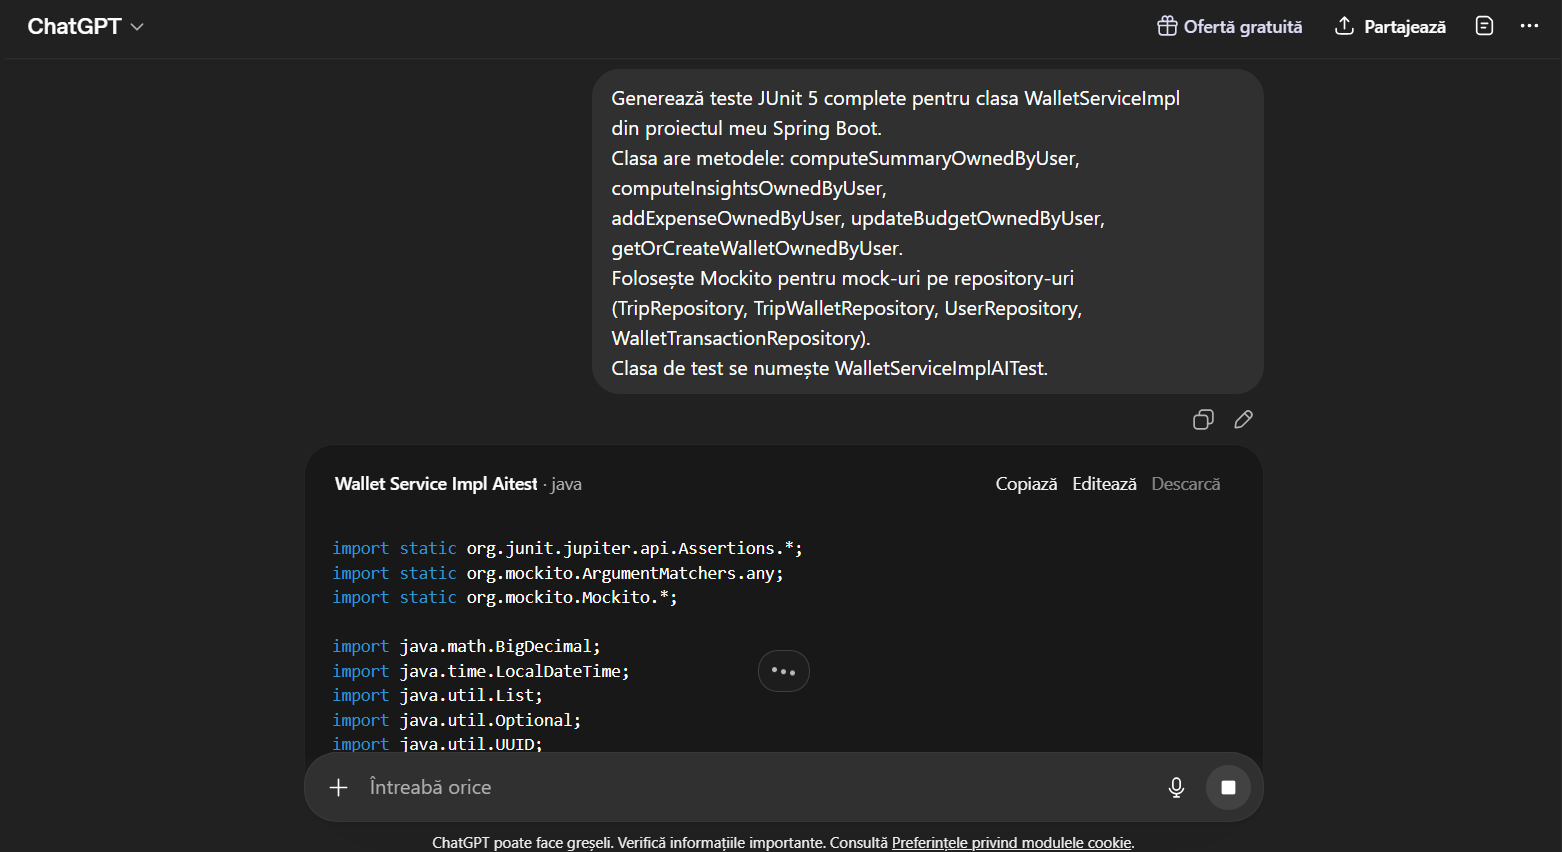
\includegraphics[width=0.85\linewidth]{ss1.png}}
    \caption{Captură de ecran cu promptul trimis în ChatGPT.}
    \label{fig:ai-prompt}
\end{figure}

\section{Răspunsul generat}

ChatGPT a returnat în aproximativ 30 de secunde o clasă de test cu adnotări corecte de Mockito (\texttt{@ExtendWith(MockitoExtension.class)}, \texttt{@Mock}, \texttt{@InjectMocks}) și aproximativ 10 metode de test, una pentru fiecare metodă publică pe care i-am menționat-o. Răspunsul complet e ilustrat în figurile \ref{fig:ai-response-1}, \ref{fig:ai-response-2} și \ref{fig:ai-response-3}.

\begin{figure}[!htb]
    \centering
    \fbox{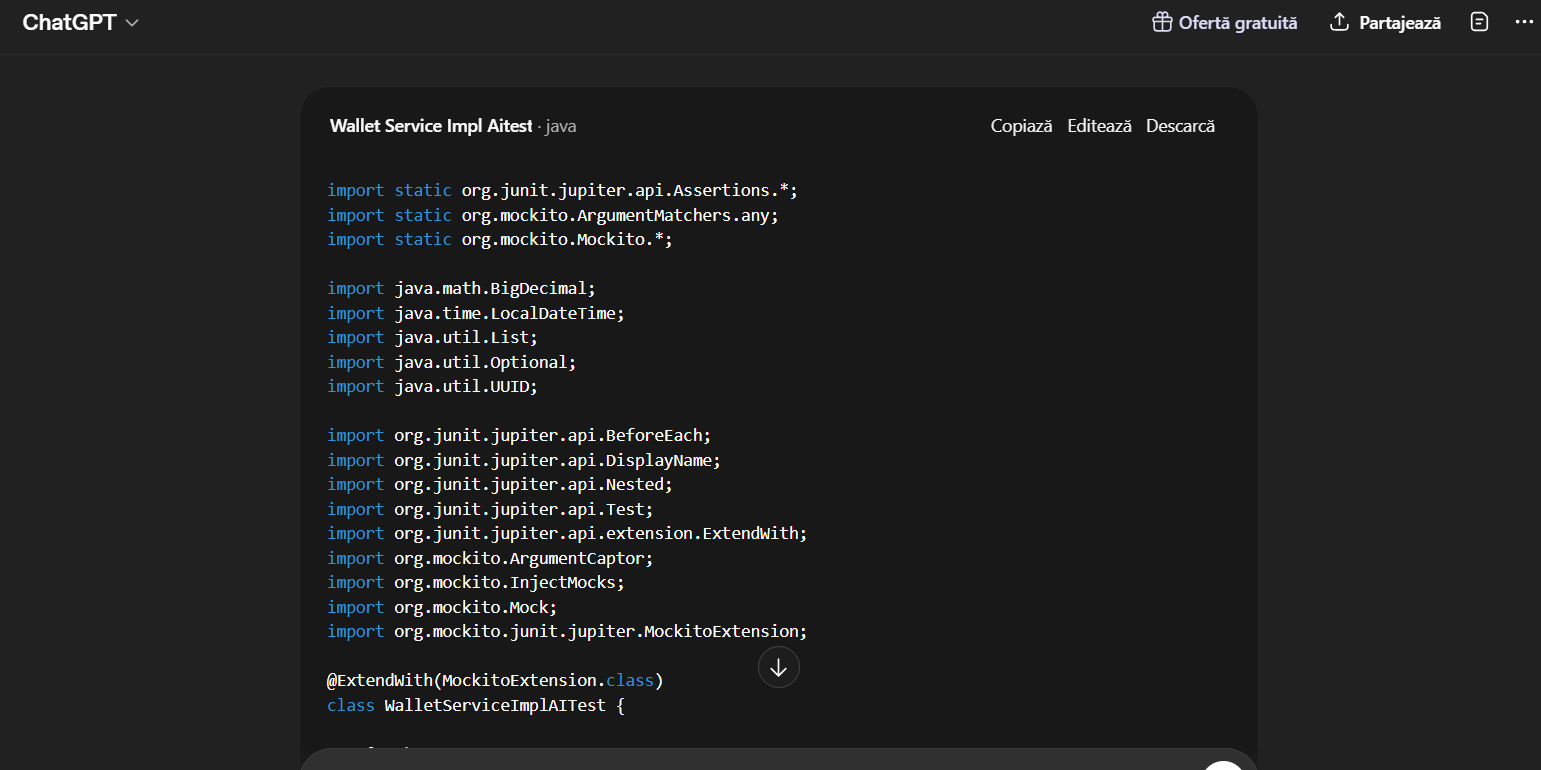
\includegraphics[width=0.85\linewidth]{ss2.png}}
    \caption{Răspunsul ChatGPT - prima parte a codului generat.}
    \label{fig:ai-response-1}
\end{figure}

\begin{figure}[!htb]
    \centering
    \fbox{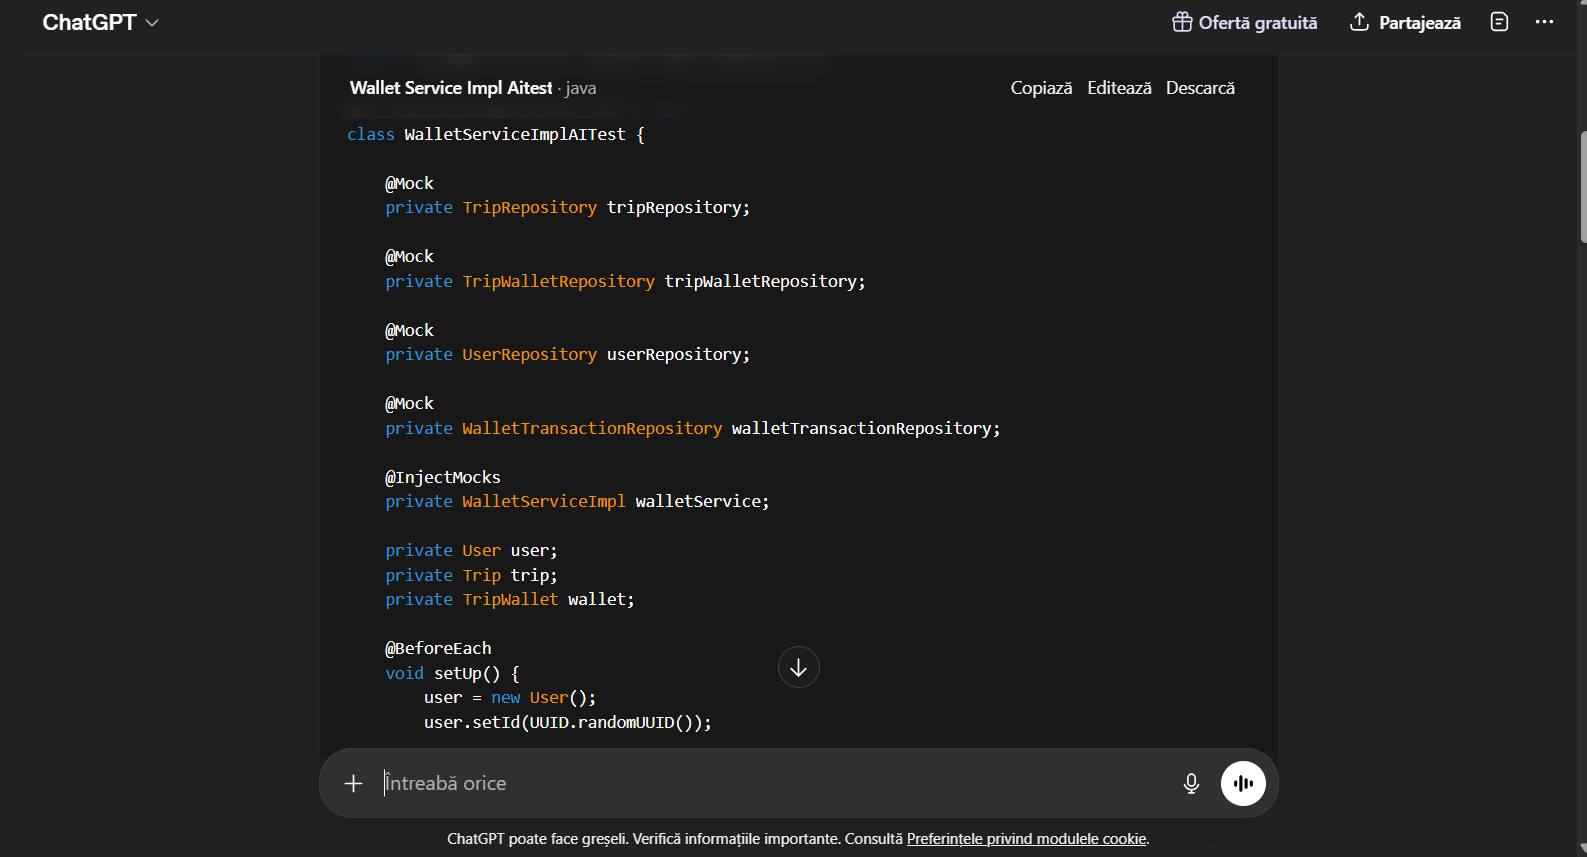
\includegraphics[width=0.85\linewidth]{ss3.png}}
    \caption{Răspunsul ChatGPT - partea a doua a codului generat.}
    \label{fig:ai-response-2}
\end{figure}

\begin{figure}[!htb]
    \centering
    \fbox{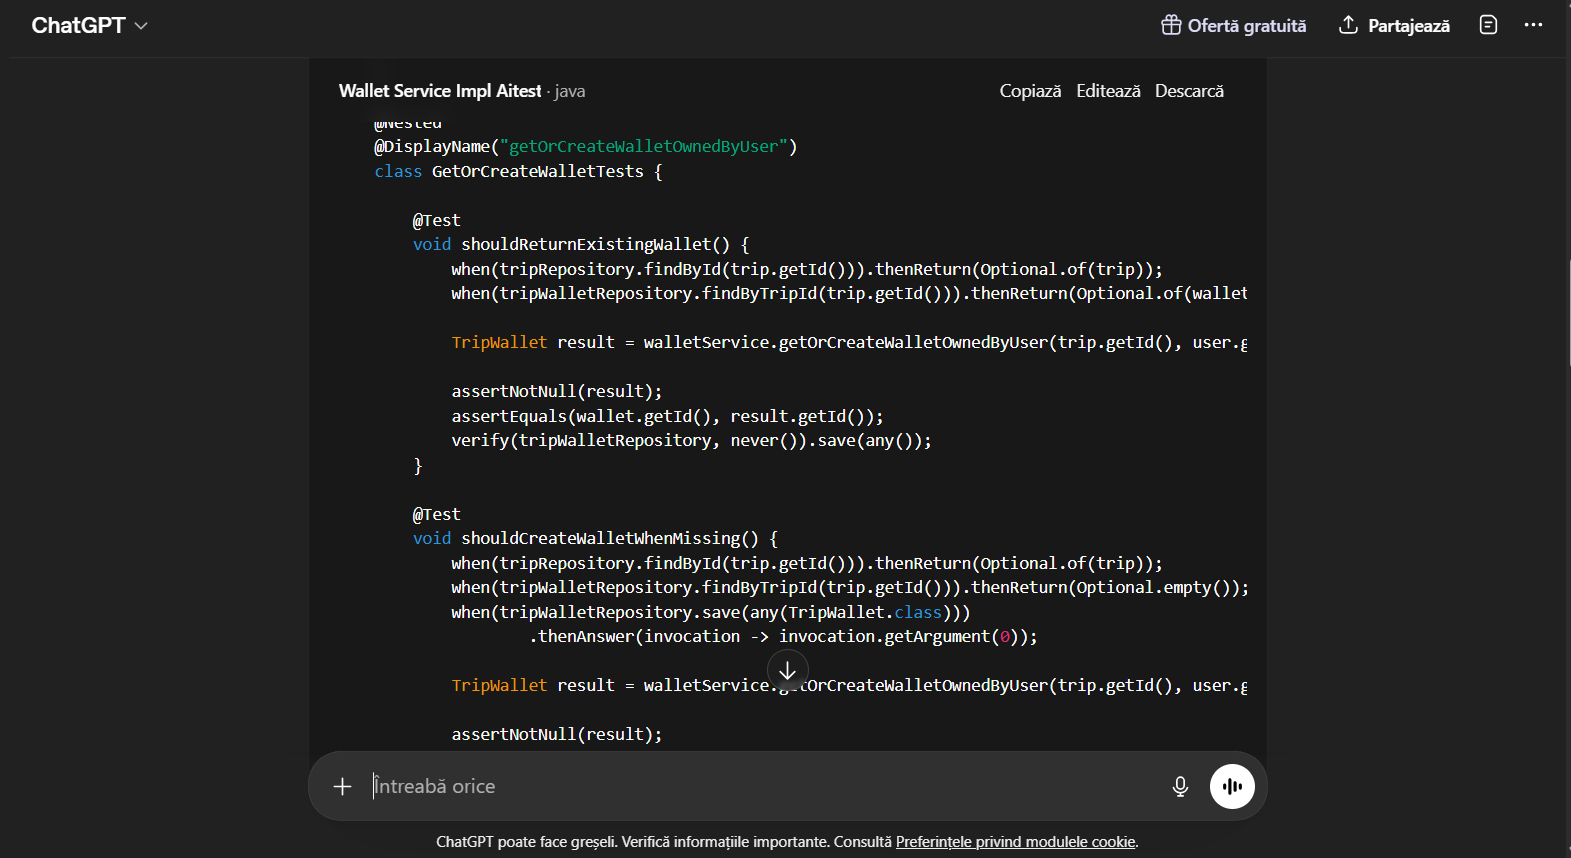
\includegraphics[width=0.85\linewidth]{ss4.png}}
    \caption{Răspunsul ChatGPT - partea finală a codului generat.}
    \label{fig:ai-response-3}
\end{figure}

\textit{Notă: imaginile \texttt{ss1.png} - \texttt{ss4.png} și \texttt{erori1.png} se află în folderul \texttt{Screenshots/} din repository și trebuie copiate în \texttt{images/} pentru ca documentul să compileze corect.}

Codul generat l-am salvat aproape neschimbat în \texttt{src/test/java/echipa13/calatorii/service/impl/WalletServiceImplAITest.java}. Singura modificare a fost adăugarea de import-uri lipsă, ca să încercăm măcar să-l compilăm. Și chiar cu import-urile adăugate, codul tot nu compilează - ceea ce e exact punctul interesant al experimentului.

\section{Rezultatul rulării: Build Failed}

\subsection{47 de erori de compilare}

Suita generată a produs \textbf{Build Failed} cu peste 40 de erori. Pentru claritate, am grupat erorile în 5 categorii distincte. Captura cu eroarea efectivă din IDE e prezentată în figura \ref{fig:ai-errors}.

\begin{figure}[!htb]
    \centering
    \fbox{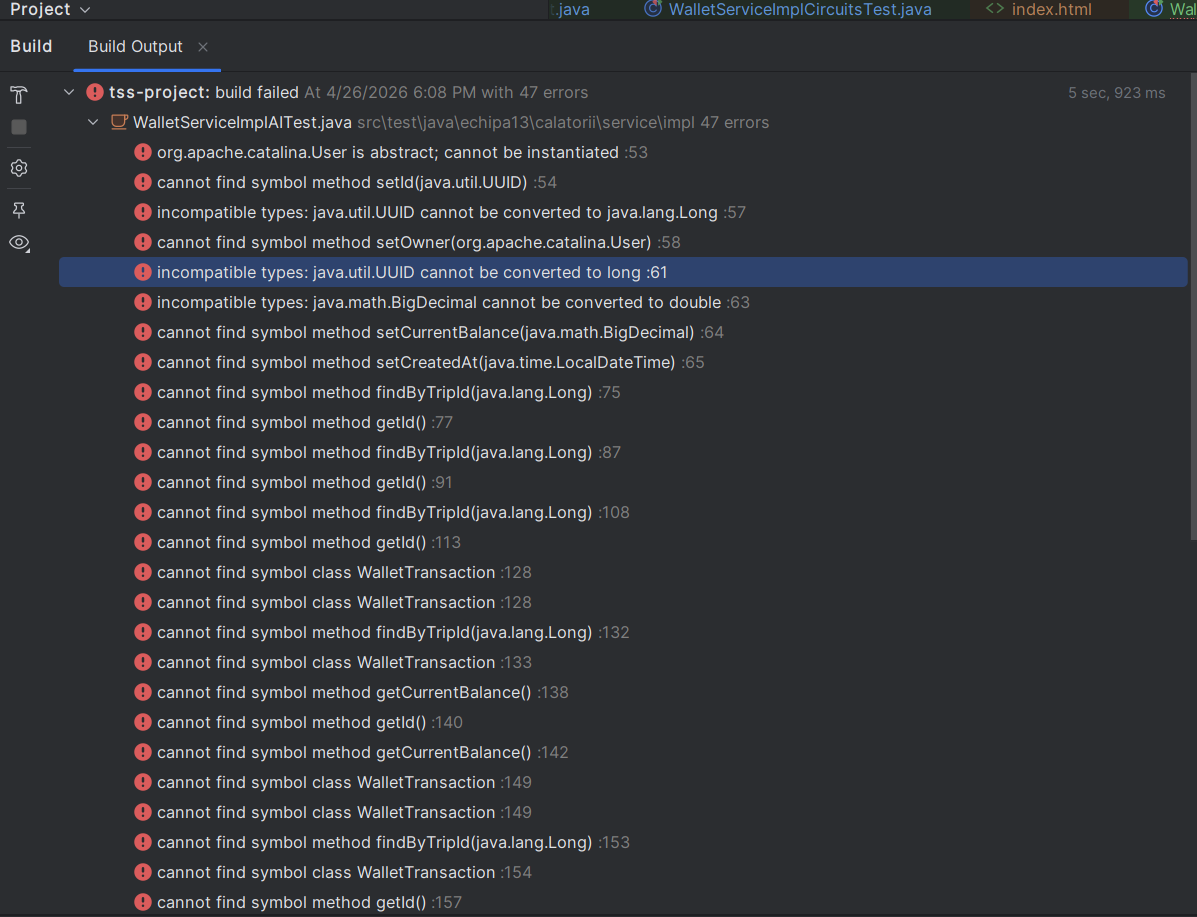
\includegraphics[width=0.85\linewidth]{erori1.png}}
    \caption{Captură din IntelliJ IDEA cu erorile de compilare ale suitei generate de AI.}
    \label{fig:ai-errors}
\end{figure}

\subsection{Categoria 1: Clase inventate, inexistente în proiect}

\begin{table}[!htb]
\centering
\caption{Clase folosite de AI vs. clasele reale din proiect.}
\label{tab:ai-classes}
\begin{tabularx}{\linewidth}{XX}
\toprule
\textbf{Clasă folosită de AI} & \textbf{Clasa reală} \\
\midrule
\texttt{WalletSummaryDto} & \texttt{WalletSummary} \\
\texttt{WalletInsightsDto} & \texttt{WalletInsights} \\
\texttt{TransactionCategory} & \texttt{WalletCategory} \\
\texttt{WalletTransaction} (cu pachet greșit) & \texttt{echipa13.calatorii.models.WalletTransaction} \\
\bottomrule
\end{tabularx}
\end{table}

AI-ul a presupus că DTO-urile au sufixul \texttt{Dto}, conform unor convenții comune în proiectele Spring, dar în proiectul nostru nu folosim acest sufix. La fel, a inventat \texttt{TransactionCategory} pe baza unui pattern frecvent, în loc de \texttt{WalletCategory} (care e termenul real folosit de modul).

\subsection{Categoria 2: Metode inventate pe modele}

\begin{table}[!htb]
\centering
\caption{Metode inventate de AI pe entitățile JPA.}
\label{tab:ai-methods}
\begin{tabularx}{\linewidth}{XX}
\toprule
\textbf{Metodă folosită de AI} & \textbf{Metoda reală} \\
\midrule
\texttt{setId(UUID)} & id-ul e gestionat de JPA, e \texttt{Long} nu \texttt{UUID} \\
\texttt{setOwner(User)} & nu există \\
\texttt{setCurrentBalance(BigDecimal)} & \texttt{setBudgetTotal(BigDecimal)} \\
\texttt{getCurrentBalance()} & \texttt{getBudgetTotal()} \\
\texttt{setCreatedAt(LocalDateTime)} & nu există ca setter public \\
\bottomrule
\end{tabularx}
\end{table}

AI-ul a presupus o convenție de naming \enquote{generică} pentru un wallet financiar (\texttt{currentBalance}), dar în domeniul nostru aplicativ termenul e \texttt{budgetTotal} - un buget alocat pentru o călătorie. Asta e o diferență semantică importantă, nu doar de naming.

\subsection{Categoria 3: Metode inventate pe repository-uri}

\begin{table}[!htb]
\centering
\caption{Metode inventate de AI pe repository-urile JPA.}
\label{tab:ai-repos}
\begin{tabularx}{\linewidth}{XX}
\toprule
\textbf{Metodă folosită de AI} & \textbf{Metoda reală} \\
\midrule
\texttt{findByTripId(Long)} (apare de 6 ori) & \texttt{findByTrip\_Id(Long)} \\
\texttt{findByWalletId(Long)} & \texttt{findByWallet\_IdOrderBySpentAtDescIdDesc(Long)} \\
\bottomrule
\end{tabularx}
\end{table}

Diferența pare minoră (un underscore), dar în Spring Data JPA contează: convenția cu \texttt{\_} indică explicit că ne referim la un câmp imbricat (proprietatea \texttt{id} a entității asociate \texttt{trip}). AI-ul a presupus convenția simplă fără underscore, care nu există în proiectul nostru.

\subsection{Categoria 4: Tipuri de date incompatibile}

AI-ul a folosit \texttt{UUID} pentru id-uri care în proiect sunt \texttt{Long}, și \texttt{double} pentru sume care în proiect sunt \texttt{BigDecimal}. A doua chestie e mai gravă pentru că \texttt{BigDecimal} e folosit explicit pentru a evita erorile de rotunjire la calcule monetare \cite{martin2008}. Înlocuirea cu \texttt{double} ar însemna o schimbare semantică reală, nu doar sintactică.

\subsection{Categoria 5: Import greșit critic}

Cea mai amuzantă eroare a fost:

\begin{lstlisting}[style=plainstyle]
org.apache.catalina.User is abstract; cannot be instantiated
\end{lstlisting}

AI-ul a importat \texttt{org.apache.catalina.User} - clasa \texttt{User} din serverul Tomcat - în locul \texttt{echipa13.calatorii.models.UserEntity} din proiect. E genul de eroare care apare când IDE-ul îți sugerează \enquote{User} și autocomplet-ul ia primul rezultat din classpath, dar AI-ul nu are acces la classpath-ul proiectului, deci a tras la sorți. A nimerit o clasă abstractă, ceea ce face și mai amuzantă situația - codul nici măcar nu se poate instanția.

\section{Comparație cantitativă suita proprie vs. suita AI}

Tabelul \ref{tab:comparison} prezintă comparația detaliată, iar figura \ref{fig:ai-vs-ours} oferă vizualizarea grafică.

\begin{table}[!htb]
\centering
\caption{Comparație detaliată suita proprie vs. suita generată de AI.}
\label{tab:comparison}
\begin{tabularx}{\linewidth}{Xll}
\toprule
\textbf{Criteriu} & \textbf{Suita proprie} & \textbf{Suita AI} \\
\midrule
Număr teste totale & $\sim$40 & $\sim$10 \\
Compilează & Da & \textbf{Nu} \\
Rulează fără erori & Da & Nu compilează \\
Statement coverage & 91\% & 0\% \\
Branch coverage & 80\% & 0\% \\
Mutation score & 60\% & 0\% \\
Ownership check acoperit & Da & \textbf{Nu} \\
Tipuri corecte (BigDecimal) & Da & folosește \texttt{double} \\
Tipuri id corecte (Long) & Da & folosește \texttt{UUID} \\
Semnături metode corecte & Da & toate greșite \\
Teste BVA (74, 75, 99, 100\%) & Da & Lipsesc \\
Teste null / invalid input & Da & Lipsesc \\
Teste circuite independente & Da & Lipsesc \\
Clase model corecte & Da & Inventate \\
API repository corect & Da & Inventat \\
Import-uri corecte & Da & \texttt{org.apache.catalina.User} \\
Duplicate / redundante & 0 & prezente \\
\bottomrule
\end{tabularx}
\end{table}

\begin{figure}[!htb]
    \centering
    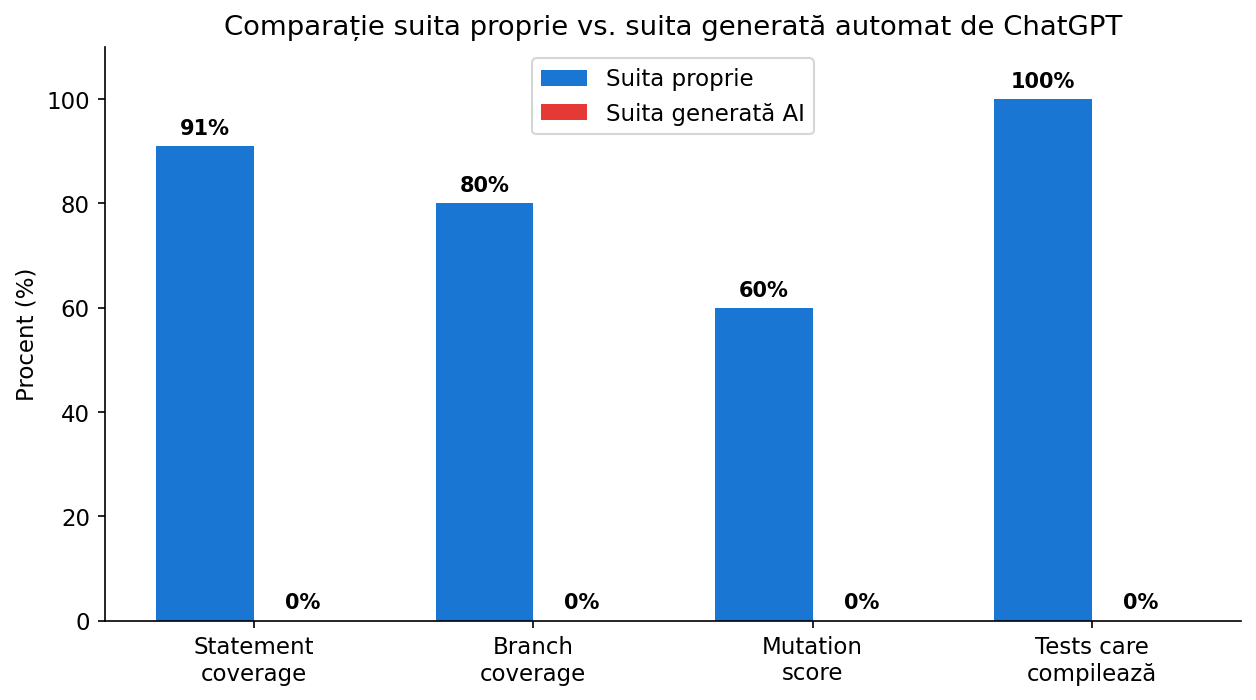
\includegraphics[width=0.85\linewidth]{10-ai-vs-ours.png}
    \caption{Comparația vizuală suita proprie vs. suita AI pe metricile principale.}
    \label{fig:ai-vs-ours}
\end{figure}

\section{Analiza diferențelor}

\subsection{Unde AI-ul ajută}

În ciuda eșecului total la nivel de compilare, AI-ul nu e complet nefolositor. Câteva aspecte unde s-a descurcat bine:

\begin{itemize}
    \item \textbf{Boilerplate rapid.} Structura de bază a clasei de test - adnotările \texttt{@ExtendWith(MockitoExtension.class)}, \texttt{@Mock}, \texttt{@InjectMocks}, metoda \texttt{@BeforeEach} - este generată corect și convențional. Dacă pornești de la zero, primești scheletul în 30 de secunde.

    \item \textbf{Identifică metodele care merită testate.} AI-ul a recunoscut corect care sunt metodele publice principale și a încercat să facă teste pentru fiecare.

    \item \textbf{Convențiile generale de naming.} Numele testelor (gen \texttt{shouldReturnSummaryWhenBudgetIsSet}) sunt rezonabile și aliniate cu stilul JUnit modern.
\end{itemize}

\subsection{Unde AI-ul greșește}

\begin{itemize}
    \item \textbf{Inventează API.} Cea mai gravă problemă: AI-ul nu cunoaște codul real, dar trebuie să producă ceva, deci \enquote{presupune} cum ar trebui să arate metodele. Ghicește pe baza unor proiecte similare pe care le-a văzut în training. Rezultatul e un cod care arată plauzibil din afară, dar nu compilează în proiectul nostru.

    \item \textbf{Ratează logica de securitate.} Toate metodele din \texttt{WalletServiceImpl} au un ownership check care aruncă \texttt{IllegalStateException} dacă userul curent încearcă să acceseze itinerariul altcuiva. AI-ul a ignorat complet acest aspect. Practic, dacă rulam codul lui pe modelul nostru real (cu ownership check), absolut toate testele ar fi aruncat \enquote{Nu ai acces la acest itinerariu}.

    \item \textbf{Confundă tipurile de date.} \texttt{Long} cu \texttt{UUID}, \texttt{BigDecimal} cu \texttt{double}. Sunt erori care la o privire rapidă par \enquote{aproape corecte}, dar care în practică schimbă semantica.

    \item \textbf{Nu aplică deloc strategii de testare structurate.} Nu există BVA, EP, Basis Path, Mutation Testing - zero. Doar câteva teste happy-path, plus unul-două cu input invalid.

    \item \textbf{Import-uri greșite.} Aici e clar că AI-ul \enquote{ghicește} pe baza numelui scurt al clasei, fără să aibă vizibilitate pe classpath-ul real.
\end{itemize}

\subsection{O observație colaterală}

Un detaliu interesant: codul generat e suficient de bine structurat încât arată ca un test bun la o privire rapidă. Dacă l-ai scana fără să-l rulezi, ai putea să crezi că e perfect funcțional. Asta e probabil cea mai mare capcană a folosirii AI-ului în testare - nu e că nu produce nimic, ci că produce ceva care pare bun fără să fie.

Rezultatul concret: dacă cineva ar fi pus codul în repository și ar fi spus \enquote{done}, build-ul s-ar fi rupt la primul \texttt{mvn compile}, iar timpul \enquote{economisit} cu AI-ul s-ar fi pierdut imediat la debug.

\section{Concluzia experimentului}

AI-ul a generat în 30 de secunde un schelet plauzibil dar nefuncțional. Codul nu compilează și nu poate fi rulat fără rescriere semnificativă. În contrast, suita proprie - care a luat câteva zile de muncă efectivă - a necesitat înțelegerea reală a implementării, alegerea deliberată a strategiilor (EP, BVA, Statement, Decision, Condition, Basis Path, Mutation) și iterare progresivă până la 91\% statement coverage și 60\% mutation score.

Concluzia principală: AI-ul e un instrument complementar, util pentru boilerplate și pentru a-ți da un punct de pornire, dar nu poate înlocui raționamentul de testare. Fără cunoașterea concretă a codului sursă și fără aplicarea conștientă a strategiilor structurate, codul generat e impresionant la suprafață și inutilizabil în practică.

Pentru viitor, scenariul realist de folosire ar fi: AI-ul îți dă scheletul + o primă rundă de teste happy-path, iar tu, ca dezvoltator, completezi BVA, edge cases, ownership checks și mutation kills. Adică AI-ul îți face partea \enquote{plicticoasă}, iar tu rezolvi partea \enquote{grea}.

Pentru completitudine, am folosit într-o oarecare măsură și \textbf{Claude} \cite{claude_ref} ca asistent în timpul dezvoltării proiectului - nu pentru a genera teste de la zero, ci pentru debug pe Mockito (când o eroare obscură pe stub-uri ne luase mai mult timp decât ne convenea), explicații pe mutanți specifici PITest și pentru recapitularea unor detalii teoretice. Asta intră tot la \enquote{AI complementar}, dar pe alt vector: ca asistent în lucrul cu suita, nu ca generator de teste.

\chapter{Concluzii}
\label{ch:concluzii}

\section{Recapitulare obiective vs. realizat}

La începutul proiectului ne-am stabilit câteva obiective concrete. Iată în ce măsură au fost atinse:

\begin{table}[!htb]
\centering
\caption{Obiectivele proiectului și realizarea lor.}
\label{tab:objectives}
\begin{tabularx}{\linewidth}{Xll}
\toprule
\textbf{Obiectiv} & \textbf{Țintă} & \textbf{Realizat} \\
\midrule
Cele 6 strategii de testare aplicate & toate & da, toate \\
Branch Coverage & $\geq$ 80\% & 80\% \\
Statement Coverage & $\geq$ 80\% & 91\% \\
Mutation Score & $\geq$ 60\% & 60\% \\
Mutanți neechivalenți omorâți explicit & $\geq$ 2 & 2 \\
Comparație cu suita AI & da & da \\
Documentație completă & da & da \\
\bottomrule
\end{tabularx}
\end{table}

Toate obiectivele au fost atinse. La unele - Statement Coverage și Mutation Score - am depășit ținta, la altele am atins exact pragul minim. Diferența vine din natura metricilor: Statement Coverage e ușor de urcat odată ce ai o suită diversificată, în timp ce Mutation Score crește mai greu pentru că cere teste \textit{stricte}, nu doar \textit{numeroase}.

\section{Ce am învățat}

\subsection{Despre proiect}

Lucrul concret pe \texttt{WalletServiceImpl} ne-a forțat să trecem prin câteva etape pe care un curs teoretic nu le poate captura:

\begin{itemize}
    \item \textbf{Alegerea claselor potrivite pentru testare.} Nu orice clasă merită toate cele șase strategii. \texttt{TripServiceImpl} ar fi fost mult mai săracă didactic, pentru că logica ei e CRUD pur. Identificarea unei clase \enquote{bogate} (cu condiții compuse, calcule, cascade de praguri) e o decizie pe care trebuie să o luăm înaintea oricărui test scris.

    \item \textbf{Distincția BVA / EP în practică.} În teorie, BVA pare doar o variantă mai paranoică a EP. În practică, BVA prinde bug-uri reale: am descoperit la un moment dat că un coleg scrisese \texttt{percent > 75} în loc de \texttt{percent >= 75}, și abia testul cu valoarea exact 75 a făcut diferența observabilă.

    \item \textbf{Mockito și \textit{strictness}}. La început, fixture-ul comun cu mock-uri în \texttt{@BeforeEach} producea \texttt{UnnecessaryStubbingException} la teste care nu foloseau toate stub-urile. Soluția a fost \texttt{@MockitoSettings(strictness = Strictness.LENIENT)}. E un detaliu mic, dar care ne-a luat câteva ore să îl identificăm, pentru că eroarea Mockito nu e foarte explicită.

    \item \textbf{PITest și mutanții echivalenți.} Nu fiecare mutant supraviețuitor e o lacună. Câțiva sunt echivalenți prin construcție și nu pot fi omorâți. Distincția între \enquote{lacună reală} și \enquote{mutant echivalent} cere atenție și, uneori, o discuție în echipă.

    \item \textbf{Trade-off-ul coverage / cod defensive.} Nu e mereu posibil să ajungi la 100\% Branch Coverage fără să compromiți codul. O verificare \texttt{if (x == null)} pe o variabilă care nu poate fi null în runtime real e o protecție utilă, dar e imposibil de testat fără să \enquote{trișezi} cu \texttt{@Spy} sau \texttt{Reflection}.
\end{itemize}

\subsection{Despre folosirea AI-ului}

Experimentul cu ChatGPT a fost mai instructiv decât ne așteptam. Nu pentru că am descoperit că AI-ul nu funcționează (lucru deja cunoscut), ci pentru că am văzut concret \textit{în ce mod} eșuează: nu cu erori grosolane care sar imediat în ochi, ci cu un cod \enquote{aproape corect} care necesită citire atentă pentru a-i identifica problemele.

Concluzia practică pe care o tragem: AI-ul e folositor ca \textit{generator de schelet} și ca \textit{asistent pentru debug}, dar nu poate înlocui raționamentul testerului uman, care:

\begin{itemize}
    \item cunoaște API-ul real al codului (nu îl ghicește);
    \item înțelege logica de business (în cazul nostru: bugetul de călătorie cu praguri 75/90/100);
    \item cunoaște regulile de securitate (ownership check);
    \item alege strategiile (BVA, EP, Mutation) conștient pe baza naturii codului.
\end{itemize}

\section{Direcții viitoare}

Dacă am avea timp suplimentar pe acest proiect, am extinde munca în următoarele direcții:

\subsection{Creșterea Mutation Score peste 75\%}

Cele două categorii de mutatori cu kill rate scăzut (\textsc{MathMutator} 0\%, \textsc{ConditionalsBoundary} 33\%) reprezintă cea mai accesibilă sursă de îmbunătățire. Cu 8-10 teste suplimentare țintite, am putea urca scorul de la 60\% la $\sim$75-80\%.

\subsection{Property-Based Testing}

Pentru calculele matematice (procent buget, burn rate, daily allowance), strategia \textit{Property-Based Testing} cu un instrument ca \textit{jqwik} \cite{jqwik_docs} ar fi un complement util la BVA. În loc să testăm valori specifice, am declara proprietăți (\enquote{procentul calculat e mereu între 0 și un infinit pozitiv}, \enquote{percent = 100 dacă și numai dacă spent = budget}) și am lăsa instrumentul să genereze sute de input-uri aleatoare.

\subsection{Integrare în CI/CD}

În prezent, suita rulează manual. Pasul natural următor ar fi integrarea într-un workflow GitHub Actions care, la fiecare push, să ruleze automat:

\begin{enumerate}
    \item \texttt{mvn test} - verifică că toate testele trec;
    \item \texttt{mvn jacoco:report} - generează raportul de coverage;
    \item \texttt{mvn pitest:mutationCoverage} pe ramurile principale;
    \item un threshold pe coverage (de ex. \enquote{Branch coverage scade sub 75\% $\Rightarrow$ build failed}).
\end{enumerate}

Această integrare ar transforma testele dintr-o etapă manuală într-un \textit{quality gate} automat, ceea ce e standard în orice proiect profesional modern.

\subsection{Testare de integrare cu Testcontainers}

Suita actuală mock-uiește integral baza de date. Pentru o testare mai realistă, am putea adăuga teste de integrare cu \textit{Testcontainers} - o bibliotecă care pornește un container Docker cu PostgreSQL real în timpul rulării testelor și permite verificări end-to-end pe layer-ul JPA. Asta ar prinde bug-uri pe care testele unitare nu le văd: erori în convențiile Spring Data, query-uri care compilează dar nu se execută corect, probleme cu lazy loading.

\section{Considerații finale}

Proiectul ne-a oferit ocazia să trecem de la teoria testării (cea învățată la curs) la practica testării (cea aplicată pe cod real). Diferența între cele două nu e mare în teorie, dar în practică se vede imediat: cursul te învață \textit{ce} strategii există, dar proiectul te învață \textit{când} să folosești fiecare, \textit{cum} să le combini, și \textit{de ce} unele teste au mai multă valoare decât altele.

Pentru noi, ca echipă, valoarea cea mai mare a venit din procesul efectiv: discuția despre care metodă merită Condition Coverage, dezbaterea despre cum desenăm CFG-ul pentru \texttt{computeDaysRemainingSafe}, momentul în care un test BVA a prins efectiv un bug \texttt{>= vs. >}.

În sfârșit, faptul că am pus suita într-un \textit{quality gate} concret (80\% Branch, 60\% Mutation) ne-a dat și o referință practică pentru viitor: când vom mai testa cod, știm acum cum arată un prag profesional. Și știm și cât de greu e să-l atingi onest, fără să forțezi metricile.


\bibliographystyle{plain}
\bibliography{bibliography}
\addcontentsline{toc}{chapter}{Bibliografie}

\appendix
\chapter{Cod sursă relevant}
\label{ch:anexe}

În această anexă sunt incluse fragmente de cod din \texttt{WalletServiceImpl} și din suita de teste, la care se face referire pe parcursul documentației. Codul complet se găsește în repository-ul GitHub al proiectului.

\section{Fragmente din \texttt{WalletServiceImpl}}

\subsection{Constructorul cu injecție de dependențe}

\begin{lstlisting}[language=Java]
@Service
public class WalletServiceImpl implements WalletService {

    private static final int WARNING_THRESHOLD_PERCENT  = 75;
    private static final int CRITICAL_THRESHOLD_PERCENT = 90;
    private static final Set<String> ALLOWED_CURRENCIES =
        Set.of("RON", "EUR");

    private final TripRepository tripRepository;
    private final TripWalletRepository tripWalletRepository;
    private final UserRepository userRepository;
    private final WalletTransactionRepository walletTransactionRepository;

    public WalletServiceImpl(TripRepository tripRepository,
                             TripWalletRepository tripWalletRepository,
                             UserRepository userRepository,
                             WalletTransactionRepository walletTransactionRepository) {
        this.tripRepository = tripRepository;
        this.tripWalletRepository = tripWalletRepository;
        this.userRepository = userRepository;
        this.walletTransactionRepository = walletTransactionRepository;
    }
    // ... metodele clasei
}
\end{lstlisting}

\subsection{Metoda \texttt{addExpenseOwnedByUser}}

\begin{lstlisting}[language=Java]
@Override
@Transactional
public WalletTransaction addExpenseOwnedByUser(
        Long tripId, String usernameOrEmail,
        BigDecimal amount, WalletCategory category,
        String title, String note,
        LocalDate spentAt, Integer dayIndex) {

    TripWallet wallet = getOrCreateWalletOwnedByUser(tripId, usernameOrEmail);

    if (amount == null || amount.compareTo(BigDecimal.ZERO) <= 0) {
        throw new IllegalArgumentException("Suma trebuie sa fie > 0.");
    }
    String safeTitle = (title == null) ? "" : title.trim();
    if (safeTitle.isBlank()) {
        throw new IllegalArgumentException("Titlul este obligatoriu.");
    }
    if (dayIndex != null && dayIndex <= 0) {
        throw new IllegalArgumentException("Ziua trebuie sa fie >= 1.");
    }

    WalletTransaction tx = new WalletTransaction();
    tx.setWallet(wallet);
    tx.setAmount(amount);
    tx.setCategory(category != null ? category : WalletCategory.OTHER);
    tx.setTitle(safeTitle);
    tx.setNote(note);
    tx.setSpentAt(spentAt != null ? spentAt : LocalDate.now());
    tx.setDayIndex(dayIndex);

    return walletTransactionRepository.save(tx);
}
\end{lstlisting}

\subsection{Metoda \texttt{computeDaysRemainingSafe}}

\begin{lstlisting}[language=Java]
private Integer computeDaysRemainingSafe(Trip trip) {
    LocalDate start = trip.getStartDate();
    LocalDate end = trip.getEndDate();

    if (start == null || end == null || end.isBefore(start)) {
        return null;
    }

    LocalDate today = LocalDate.now();
    if (today.isAfter(end)) {
        return 0;
    }
    if (today.isBefore(start)) {
        return (int) (ChronoUnit.DAYS.between(start, end) + 1);
    }
    return (int) (ChronoUnit.DAYS.between(today, end) + 1);
}
\end{lstlisting}

\section{Fragmente din suita de teste}

\subsection{Configurare comună}

\begin{lstlisting}[language=Java, caption={Schelet din \texttt{...EquivalenceTest.java}}]
@ExtendWith(MockitoExtension.class)
@MockitoSettings(strictness = Strictness.LENIENT)
public class WalletServiceImplEquivalenceTest {

    @Mock private TripRepository tripRepo;
    @Mock private TripWalletRepository walletRepo;
    @Mock private UserRepository userRepo;
    @Mock private WalletTransactionRepository txRepo;

    @InjectMocks private WalletServiceImpl service;

    private TripWallet wallet;
    private Trip trip;
    private final Long tripId = 10L;
    private final String login = "user@test.com";

    @BeforeEach
    public void setUp() {
        UserEntity user = new UserEntity();
        user.setId(1L);
        user.setEmail(login);

        trip = new Trip();
        trip.setId(tripId);
        trip.setUser(user);
        trip.setStartDate(LocalDate.of(2026, 4, 15));
        trip.setEndDate(LocalDate.of(2026, 4, 22));

        wallet = new TripWallet();
        wallet.setId(100L);
        wallet.setTrip(trip);
        wallet.setBudgetTotal(new BigDecimal("1000"));
        wallet.setCurrency("RON");

        when(userRepo.findByEmail(login)).thenReturn(user);
        when(tripRepo.findById(tripId)).thenReturn(Optional.of(trip));
        when(walletRepo.findByTrip_Id(tripId))
            .thenReturn(Optional.of(wallet));
    }
}
\end{lstlisting}

\subsection{Test pentru clasa de echivalență P4 (sumă invalidă)}

\begin{lstlisting}[language=Java]
@Test
public void testAdaugaCheltuiala_SumaNegativa_AruncaExceptie() {
    BigDecimal sumaNegativa = new BigDecimal("-10");
    assertThrows(IllegalArgumentException.class, () ->
        service.addExpenseOwnedByUser(tripId, login,
            sumaNegativa, WalletCategory.FOOD,
            "Pranz", null, LocalDate.now(), 1));

    verify(txRepo, never()).save(any());
}
\end{lstlisting}

\subsection{Test pentru BVA pe pragul de 75\%}

\begin{lstlisting}[language=Java]
@Test
public void testSumar_ExactPragAtentie_75LaSuta() {
    wallet.setBudgetTotal(new BigDecimal("100"));
    when(txRepo.sumAmountByWalletId(any()))
        .thenReturn(new BigDecimal("75"));

    WalletSummary summary =
        service.computeSummaryOwnedByUser(tripId, login);

    assertEquals(75, summary.getPercent());
    assertEquals(WalletSummary.Status.ATENTIE, summary.getStatus());
    assertEquals(new BigDecimal("25.00"),
        summary.getRemaining().setScale(2));
}
\end{lstlisting}

\subsection{Test pentru Condition Coverage cu 3 operanzi OR}

\begin{lstlisting}[language=Java]
@Test
public void testStergere_OwnershipCheck_ConditionCoverage() {
    Long txId = 42L;

    // Caz 1: tranzactie cu wallet null -> primul operand TRUE
    WalletTransaction txCuWalletNull = new WalletTransaction();
    txCuWalletNull.setId(txId);
    txCuWalletNull.setWallet(null);
    when(txRepo.findById(txId)).thenReturn(Optional.of(txCuWalletNull));
    assertThrows(IllegalStateException.class, () ->
        service.deleteTransactionOwnedByUser(tripId, login, txId));

    // Caz 2: tranzactie cu id null -> al doilea operand TRUE
    WalletTransaction txCuIdNull = new WalletTransaction();
    txCuIdNull.setWallet(wallet);
    when(txRepo.findById(txId)).thenReturn(Optional.of(txCuIdNull));
    assertThrows(IllegalStateException.class, () ->
        service.deleteTransactionOwnedByUser(tripId, login, txId));

    // Caz 3: id-uri diferite -> al treilea operand TRUE
    TripWallet altWallet = new TripWallet();
    altWallet.setId(999L);
    WalletTransaction txCuIdGresit = new WalletTransaction();
    txCuIdGresit.setId(txId);
    txCuIdGresit.setWallet(altWallet);
    when(txRepo.findById(txId)).thenReturn(Optional.of(txCuIdGresit));
    assertThrows(IllegalStateException.class, () ->
        service.deleteTransactionOwnedByUser(tripId, login, txId));

    // Caz 4: toate operandele FALSE -> stergere reusita
    WalletTransaction txValid = new WalletTransaction();
    txValid.setId(txId);
    txValid.setWallet(wallet);
    when(txRepo.findById(txId)).thenReturn(Optional.of(txValid));
    service.deleteTransactionOwnedByUser(tripId, login, txId);
    verify(txRepo).delete(txValid);
}
\end{lstlisting}

\subsection{Test țintit pentru mutantul \textsc{MathMutator}}

\begin{lstlisting}[language=Java]
@Test
public void should_kill_percent_math_mutations() {
    wallet.setBudgetTotal(new BigDecimal("200"));
    when(txRepo.sumAmountByWalletId(any()))
        .thenReturn(new BigDecimal("50"));

    WalletSummary s = service.computeSummaryOwnedByUser(tripId, login);

    // 50 / 200 * 100 = 25%. Daca multiply si divide
    // sunt schimbate intre ele, calculul va da o valoare
    // diferita (in particular, 0 dupa rotunjire).
    assertEquals(25, s.getPercent());
}
\end{lstlisting}

\subsection{Test pentru Circuits pe \texttt{computeDaysRemainingSafe}}

\begin{lstlisting}[language=Java]
@Test
public void testCircuiteIndependente_computeDaysRemainingSafe() {
    // C1: start = null
    trip.setStartDate(null);
    trip.setEndDate(LocalDate.now().plusDays(5));
    WalletInsights i1 = service.computeInsightsOwnedByUser(tripId, login);
    assertNull(i1.getDaysRemaining());

    // C2: end = null
    trip.setStartDate(LocalDate.now());
    trip.setEndDate(null);
    WalletInsights i2 = service.computeInsightsOwnedByUser(tripId, login);
    assertNull(i2.getDaysRemaining());

    // C3: end < start (interval invalid)
    trip.setStartDate(LocalDate.now().plusDays(10));
    trip.setEndDate(LocalDate.now().plusDays(5));
    WalletInsights i3 = service.computeInsightsOwnedByUser(tripId, login);
    assertNull(i3.getDaysRemaining());

    // C4: today > end (calatorie incheiata)
    trip.setStartDate(LocalDate.now().minusDays(20));
    trip.setEndDate(LocalDate.now().minusDays(10));
    WalletInsights i4 = service.computeInsightsOwnedByUser(tripId, login);
    assertEquals(0, i4.getDaysRemaining());

    // C5: today < start (calatorie viitoare)
    trip.setStartDate(LocalDate.now().plusDays(3));
    trip.setEndDate(LocalDate.now().plusDays(9));
    WalletInsights i5 = service.computeInsightsOwnedByUser(tripId, login);
    assertEquals(7, i5.getDaysRemaining());

    // C6: caz normal (calatorie in desfasurare)
    trip.setStartDate(LocalDate.now().minusDays(2));
    trip.setEndDate(LocalDate.now().plusDays(4));
    WalletInsights i6 = service.computeInsightsOwnedByUser(tripId, login);
    assertEquals(5, i6.getDaysRemaining());
}
\end{lstlisting}

\section{CFG pentru \texttt{addExpenseOwnedByUser}}

Pentru completitudine, mai jos e prezentat și CFG-ul pentru \texttt{addExpenseOwnedByUser} (figura \ref{fig:cfg-addExpense}), care e cea mai testată metodă din clasa noastră.

\begin{figure}[!htb]
    \centering
    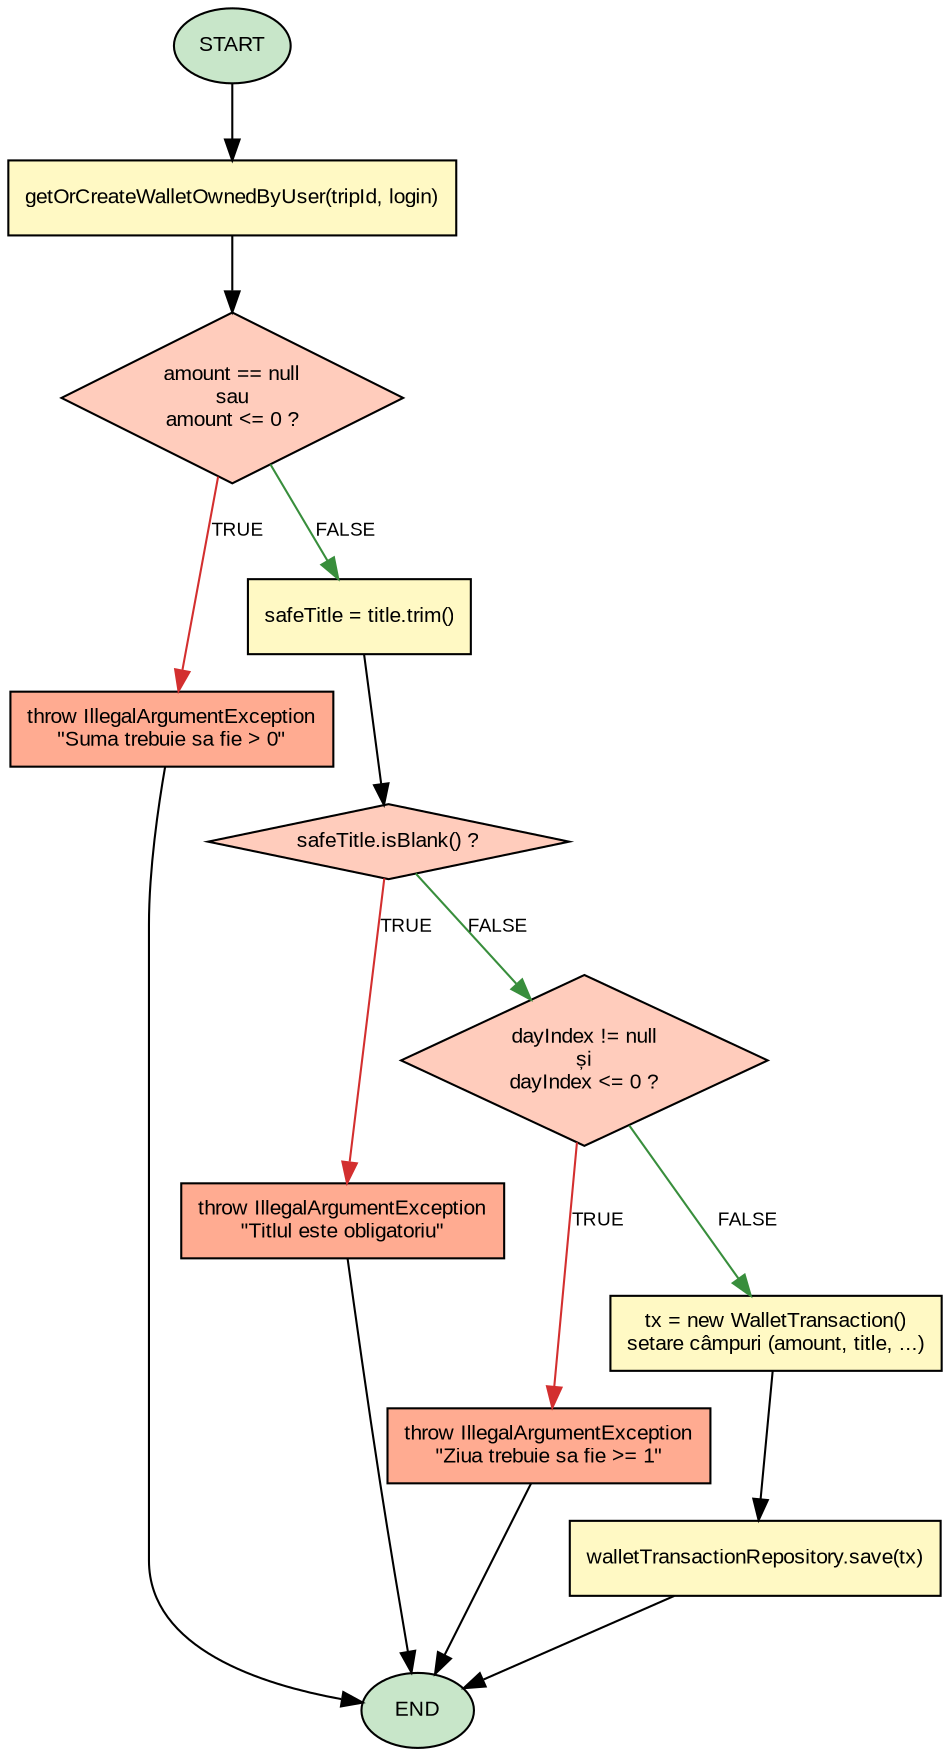
\includegraphics[width=0.7\linewidth]{03-cfg-addExpense.png}
    \caption{CFG pentru \texttt{addExpenseOwnedByUser}: trei decizii principale (sumă, titlu, dayIndex) cu trei branch-uri de eroare și o cale de succes.}
    \label{fig:cfg-addExpense}
\end{figure}


\end{document}
